\documentclass[12pt]{article}

\usepackage{aer,amssymb,amsmath,amsfonts,booktabs,eurosym,float,geometry,ulem,graphicx,caption,color,setspace,sectsty,comment,footmisc,caption,pdflscape,subfigure,subcaption,hyperref,mathtools,appendix,ragged2e,longtable,dcolumn,adjustbox,tabularx,enotez,hyperref,xcolor}
\usepackage[flushleft]{threeparttable}
\usepackage[utf8]{inputenc}
\usepackage [english]{babel}
\usepackage [autostyle, english = american]{csquotes}
\MakeOuterQuote{"}

\normalem

\usepackage{natbib}


\onehalfspacing
\newtheorem{theorem}{Theorem}
\newtheorem{corollary}[theorem]{Corollary}
\newtheorem{proposition}{Proposition}
\newenvironment{proof}[1][Proof]{\noindent\textbf{#1.} }{\ \rule{0.5em}{0.5em}}

\newtheorem{hyp}{Hypothesis}
\newtheorem{subhyp}{Hypothesis}[hyp]
\renewcommand{\thesubhyp}{\thehyp\alph{subhyp}}

\newcommand{\red}[1]{{\color{red} #1}}
\newcommand{\blue}[1]{{\color{blue} #1}}

\newcolumntype{L}[1]{>{\raggedright\let\newline\\arraybackslash\hspace{0pt}}m{#1}}
\newcolumntype{C}[1]{>{\centering\let\newline\\arraybackslash\hspace{0pt}}m{#1}}
\newcolumntype{R}[1]{>{\raggedleft\let\newline\\arraybackslash\hspace{0pt}}m{#1}}

\geometry{left=1.0in,right=1.0in,top=1.0in,bottom=1.0in}

\begin{document}

\bibliographystyle{aer}
\setcitestyle{round,semicolon}

\begin{titlepage}
\title{International Migration Amid Insurgent Violence\\
(Job Market Paper)}
\author{\textbf{Ryan Ellis}\thanks{School of Economics, Georgia Institute of Technology, Atlanta, GA 30332. I thank Robert Gonzalez, Daniel Dench, Stephen O'Connell, Olga Shemyakina, and Max Rosenthal for their comments and guidance. I am also grateful to Dylan Brewer, Tibor Besedes, Mayra Pineda-Torres, Austin Wright, Jean-François Maystadt, Giovanni Peri, Catalina Amuedo-Dorantes, Xiao Hui Tai, Aidan Milliff, Mohammad Isaqzadeh, and participants at the 2024 Annual Meeting for Empirical Studies of Conflict, the 2024 UNU-WIDER Development Conference, and the 2023 AlianzaMX Summer School on the Economics of Migration.}}
\date{\today \\
\href{https://www.ryandouglasellis.com/research}{\color[HTML]{0000EE}[Link to most recent version]}}
\maketitle

\begin{abstract}
\noindent How does exposure to insurgent violence influence an individual’s decision to leave their home country? To answer this question, I combine anonymous mobile call detail records with data on the location and timing of violent events in Afghanistan to identify individual exposures to insurgent actions. I propose a novel method to detect international migration events that combines inferences from users' spatiotemporal movement patterns and episodes of sample attrition. Estimating a migration choice model reveals that a unit increase in the rate of monthly exposures to insurgent violence raises the odds of international migration by 6.4\%. I show evidence that this effect is due more to extreme, high-casualty events than to the gradual accumulation of exposures to common, low-intensity events. In contrast, \textit{internal} migration is unaffected across all violence types and intensities. I explore how wealth and employment composition might explain the differential effects. These findings provide policy-relevant insights into how potential migrants respond to insurgent violence.

%\noindent How does exposure to insurgent violence influence an individual's decision to leave their home country? One major challenge of empirical migration research is the simple fact that most micro-level data are constrained by national borders. While the proliferation of passively collected digital trace data has led to novel measures of within-country migration, questions of cross-border movement remain difficult to study in many contexts. This paper develops the first general method to infer international migration events from a type of anonymous cell phone metadata commonly used in empirical research. I propose a set of spatial and temporal criteria to categorize attrition episodes that are plausibly due to users emigrating through known land border crossings. I then apply the classification method to data from a major mobile network operator in Afghanistan, linked to military records of violent events during an active period of the Taliban insurgency. Upon identifying migrations, I estimate a displacement choice model that reveals increasing odds of international migration with additional exposures to violence, as expected. The impact of high-casualty events is greater by an order of magnitude, though the smaller effect of accumulated exposures remains persistent. In contrast, the odds of \textit{internal} migration are unaffected by the same changes in exposure rate. These results provide policy-relevant insight into the complex ways individuals choose to respond to insurgent violence near home. \\
\vspace{.5cm}

\noindent\textbf{Keywords:} Migration, Conflict, Big Data
\hfill \noindent \textbf{JEL Codes:} 015, D91, D74

\bigskip
\end{abstract}
\setcounter{page}{0}
\thispagestyle{empty}
\end{titlepage}





\doublespacing

%%%%%%%%%%%%%%%%%%%%%%%%%%%%%%%%%%%%%%%%%%%%%%%%%%%%%%%%
%%%%%%%%%%%%%%%%%%%%%%%%%%%%%%%%%%%%%%%%%%%%%%%%%%%%%%%%

\section{Introduction} \label{sec:introduction}
%%%%%%%%%%%%%%%%%%%%%%%%%%
% Motivation 
%%%%%%%%%%%%%%%%%%%%%%%%%%

In 2023, approximately 117.3 million people worldwide lived displaced from home due to conflict, violence, human rights abuses, or persecution \citep{united_nations_high_commissioner_for_refugees_global_2024}. Rates of violent conflict continue to rise globally, creating conditions that drive even more people to leave their homes \citep{world_bank_world_2020}. Migration due to violence is not only a critical humanitarian concern, but also a polarizing political issue in both host and origin countries. For these reasons, an improved understanding of the nature of violent conflict as a migration push factor is critical, especially for migration across international boundaries. Despite its importance, research on the issue remains limited. This gap exists for two primary reasons. First, external migration is challenging to measure in data-scarce environments, such as those where violence-driven migration is often most prevalent. Second, it is difficult to reliably measure individual-level exposure to violence.\par

%%%%%%%%%%%%%%%%%%%%%%%%%
% Resarch Q and brief description
%%%%%%%%%%%%%%%%%%%%%%%%%

This paper studies the impact of exposure to violence on an individual's decision to migrate in the context of Afghanistan during a peak period of the Taliban insurgency, 2010-2012. In doing so, I introduce a novel approach to the data challenges described above. First, using high frequency call detail records from a major Afghan mobile network operator to approximate the daily locations of individuals, I identify cross-border migration events through a set of spatial and temporal classifying criteria related to phone users' movement patterns at the time of their attrition from the data. To my knowledge, this paper is the first to use call detail records to infer migration events across international borders. Second, I match user locations with previously classified, geolocated, and time-stamped significant actions event data (SIGACT) to generate an individual-by-day measure of exposure to insurgent violence. I estimate a discrete choice model of migration that is flexible to the inclusion of both internal and international locations.\par

I find that a unit increase in an individual's monthly rate of exposure to insurgent violence is associated with an increase in the odds of migrating internationally between 6.3\% and 19.3\%. The estimated range is illustrative of a conservative bounding exercise in my classification of migrants with call detail records, which requires careful researcher choice of tuning parameters. When allowing for a larger radius of exposure to violent events (moving from 5km to 20km), the effect on migration shrinks to an odds increase between 0 and 2.6\%. I explore possible response heterogeneity by restricting violence to especially high-casualty events (10+ killed or wounded), revealing estimated odds increases that are higher by more than an order of magnitude--from 6.3\% for all events, to 90\% for high-casualty events--suggesting that the low-level accumulation of exposure may be much less salient to decision-makers than single extreme shocks.\par
 
Interestingly, there is no discernible effect on rates of internal migration subject to the same changes in exposure, even in response to high-casualty events. I explore the role of income and other determinants to explain the differential effects, showing that mobility (a proxy for income) increases the odds of internal migration only. The main results are robust to expanding the location choice set to include internal and international destinations. I provide additional consistent evidence via a Cox proportional-hazards model, allowing an interpretation that is sensitive to time.\par
 
The majority of previous micro-level work on violence and migration has been limited by national borders, within which only internal migration is observable. When one leaves their country of origin, they are no longer observable in its administrative datasets, censuses, or national surveys. Similarly, data collected by host countries rarely contain the geographic detail necessary to construct meaningful measures of a migrant's previous life in their country of origin.\footnote{Exceptions include surveys produced by scholars for the express purpose of studying immigration in specific contexts, such as the \href{https://oprdata.princeton.edu/Archive/MMP/}{Mexican Migration Project}.} A related literature makes use of aggregate-level country statistics of the stock and flow of migrants to estimate determinant factors, but is less appropriate for individual or household-level decision models.\footnote{See \cite{tai_mobile_2022} for a recent example that also uses digital trace data, focused on internal migration. See \cite{shaver_causes_2024} for an aggregate-level approach, and \cite{buggle_refugees_2023} for a creative solution using historical records.} By joining the benefits of aggregate-level studies that observe true migration events with those of micro-level studies that observe pre-migration histories, this project provides a valuable contribution to our understanding of the role of violence in migration decisions. The classification method for identifying international migration events is itself a further contribution of the paper, as it is generalizable for use across migration contexts.\par


 


% Digital trace data, a category of passively collected data generated by the use of cell phones, web applications, and other consumer technologies, offers a way around the issue. 
 

%%%%%%%%%%%%%%%%%%%%%%%%%
One recent meta-analysis of both micro-level and aggregate-level migration scholarship notes that a majority of studies find violence to be central among displacement push-factors, while the economic or policy-related pull factors of host locations may be less important \citep{shaver_causes_2024}. Several examples find consistently positive effects of violence on migration across distinct settings \citep{kirchhoff_displacement_2002,ibanez_civil_2008,orozco-aleman_drug_2018,buggle_refugees_2023}. While the overall direction of this effect is obvious in a rational choice framework, many studies have documented heterogeneous and even counter-intuitive results. \cite{bohra-mishra_individual_2011} show evidence for a nonlinear threshold theory of violence--that at low levels, exposures to violence actually reduce the likelihood of leaving, until a threshold is met and the sign switches. \cite{milliff_big-data_2022} show how measures of social centrality can have a strong moderating influence on other determinants of migration, including exposures to violence. Notably for this project, \cite{basu_violence_2017} find that violent events can influence international movement, but appear to be unrelated to internal migration decisions. This paper provides evidence that supports their conclusion.\par

%%%%%%%%%%%%%%%%%%%%%%%%%
%%%%%%%%%%%%%%%%%%%%%%%%%
Other recent works have turned to nontraditional data in settings where censuses and surveys are scarce or unsatisfactory, borrowing from information and communications technology, demography, physics, and other fields where necessary. \cite{blumenstock_inferring_2012} first developed a method to infer internal migration events from call detail records. The methods of measurement developed in that paper have since been updated or refined \citep{chi_general_2020,blumenstock_migration_2023} and used in subsequent research related to violence and migration (including the aforementioned work of \cite{milliff_big-data_2022}). \cite{tai_mobile_2022} finds violence plays a vital but nuanced role in internal migration episodes in Afghanistan. The authors find the odds of migration increase much more for high-casualty events, especially those credited to insurgent groups who were perceived to be more extreme. While these previous works focused exclusively on using call detail records to infer internal migration, this paper presents a novel method for using CDR to identify external migration. This creates a valuable link for migration researchers attempting to match post-migration outcomes to individual characteristics and behaviors in their country of origin.

%%%%%%%%%%%%%%%%%%%%%%%%%

% The bulk of empirical migration research utilizes aggregate-level data on migration intentions, micro-level surveys of families left behind, or proxy methods to identify immigrants in host-country administrative data. The benefits of digital trace data collected from phones, apps, or websites, are clear: they reveal the actual movement of people, as opposed to a surveyed intention, and they can be collected almost instantly. This allows policymakers to respond quickly in any setting with a human mobility component, like natural disasters or disease outbreaks.

%%%%%%%%%%%%%%%%%%%%%%%%%
% Roadmap
%%%%%%%%%%%%%%%%%%%%%%%%%

The remainder of the paper is structured as follows: Section \ref{sec:background} provides historical background on violence in Afghanistan. Section \ref{sec:data} describes the data and reports summary statistics. Section \ref{sec:method} introduces the classifying criteria for cross-border migration events. Section \ref{sec:model} outlines a model for displacement choice, and \ref{sec:empirics} contains a framework for estimation, as well as the main results. Section \ref{sec:conclusion} discusses the relevance of the contributions to researchers and policymakers, then concludes.

%%%%%%%%%%%%%%%%%%%%%%%%%%%%%%%%%%%%%%%%%%%%%%%%%%%%%%%%%%%%
%%%%%%%%%%%%%%%%%%%%%%%%%%%%%%%%%%%%%%%%%%%%%%%%%%%%%%%%%%%%

\section{Setting} \label{sec:background}
\subsection{Historical background}

The setting of this study is Afghanistan from the end of 2010 until mid-2012. The half-century prior to this period was characterized by almost constant war, both internally and with outside actors. In 1978, an Afghan civil war was absorbed into the broader international landscape of the Cold War. The Soviet Union invaded, occupied, and waged war in Afghanistan against Islamist rebel groups supported by the United States and Pakistan, among others. Estimates of Afghan civilian deaths are generally around 1.5 to 2 million in the period until 1989, with up to 6 million forcibly displaced as refugees, mostly to Iran and Pakistan, and an additional 5 million displaced internally \citep{kakar_afghanistan_1997}. The country still has not recovered even half of the 6 million displaced during its Soviet era, and return migration has stalled in recent decades. As of 2021, only Syria had more of its citizens living as refugees in other nations \citep{united_nations_high_commissioner_for_refugees_unhcr_2022}. Following the collapse of the Soviet Union, several groups attempted to gain power in the vacuum left behind. The Taliban, a militant group of Islamist scholars and former anti-Soviet fighters, first took control of Kandahar City in 1995 following a surprise attack. With support from Pakistan’s Inter-Service Intelligence (ISI), they quickly gained popularity and territory, establishing themselves as the leaders of a renamed Islamic Emirate of Afghanistan one year later in 1996. They ruled harshly until 2001, when they were ousted by a U.S.-supported coalition that included Afghanistan’s Northern Alliance.\par

\subsection{The Taliban insurgency}

During the 2000s, the Taliban regrouped in hiding, and by 2010 were an active and threatening insurgency, prompting the Obama administration to commit 100,000 troops to the country \citep{stanford_university_mapping_2018}. This is the approximate window during which the events of this study take place. In the south near the once \textit{de facto} capital Kandahar, in population centers near Kabul, and in the eastern provinces patrolled by the violent offshoot Haqqani network, the Taliban were destructive and relentless. They employed a deliberate strategy to make the state appear weak. They threatened voters, then followed through with violence during elections. They attacked city centers that offered no feasible territorial gain, chosen only to spread terror and sow mistrust. They used surprise violence to erode public faith in local and national government, and to humiliate the cooperating international coalition \citep{condra_logic_2018}. \par

The majority of Afghan refugees from both the Soviet period and the Taliban insurgency live in Pakistan and Iran. The next most common host country that also shares a land border with Afghanistan is Tajikistan, shown for reference in Figure \ref{fig:unhcr}.\footnote{Millions of asylum-seekers from Afghanistan also reside in nations across the world, primarily in Europe, but they fall outside the scope of this study.} While the stock of refugees began decreasing around 2010, many continued to displace across borders, even as return migration in certain regions outpaced the rate of exits. The border dividing Pakistan and Afghanistan is notable in a migration study, as its establishment in 1893 created an artificial divide through the lands of the Pashtun people. Many refuse to recognize the border (called the Durand Line). The shared culture, language, and history of this region are all obvious positive determinants for migration choice, especially if there are different rates of violence on either side of the border.

\begin{figure}[h]
    \centering
    \caption{Millions of Afghan refugees in bordering countries}
    \includegraphics[width=0.8\linewidth]{analysis/results/figures/unhcr_refugees_tsline.png}
    \vspace{0.25cm}
    \caption*{\small \textit{Notes:} The stock of Afghan refugees in Pakistan, Iran, and Tajikstan from 1995 to 2015. Data are from the \cite{united_nations_high_commissioner_for_refugees_unhcr_2022}. The units on the vertical axis represent millions.}
    \label{fig:unhcr}
\end{figure}

While the Taliban insurgency is a unique setting, its human and economic costs are generalizable to other conflicts and crises. The World Bank estimates that by 2030, two thirds of the world's population could live in settings characterized by fragility, conflict, and violence \citep{world_bank_world_2020}. A global pandemic and the return of land invasion-style warfare between nation-states are two recent shocks that threaten the stability and well-being of vulnerable populations. It is urgent that conflict and development research adopt the full array of new tools and methods at its disposal to address these issues. That includes new sources of data, especially in settings where administrative data are scarce. Afghanistan, for instance, last conducted an official census in 1979. Satellite imagery, social media metadata, cell phone records, and other digital trace data have unique limitations, some more obvious than others, as discussed below. Even still, their scope, consistency, and ubiquitous presence in almost every country make them helpful in diagnosing and solving policy issues.


\section{Data} \label{sec:data}
\subsection{SIGACT}

There are two primary data sources for this study. The first is the violent events dataset, compiled from the U.S. Department of Defense's Significant Activities database (SIGACT) during \textit{Operation Enduring Freedom}, the department's name for both the war in Afghanistan and the more broadly defined US war against terrorism. SIGACT data in Afghanistan were recorded by Afghanistan's own military and police units, as well as by cooperating forces of the North Atlantic Treaty Organization's (NATO) International Security Assistance Force (ISAF).\par

Violent events are categorized by type of attack (direct fire, indirect fire, improvised explosive device (IED), surface-to-air attack, and more) and are catalogued with high temporal and spatial precision. They include instances of engagement between insurgents and the ISAF counterinsurgency, as well as events of civilian or built-environment targeting. The systematic recording procedure provides an advantage in accuracy and completeness over databases of violent events compiled from media reports \citep{condra_logic_2018}. SIGACT data from Afghanistan have been used in conflict research since 2015 \citep{sexton_aid_2016,trebbi_insurgent_2020,blumenstock_violence_2024,grasse_courting_2024}. Figure \ref{fig:sigacts_by_district} illustrates the geographical spread of insurgent violence coded in SIGACT during the sample period of this study, which is concentrated along a ring shaped network of highways connecting population centers, with less activity in the country's remote center.\\

\begin{figure}[H]
    \centering
    \caption{SIGACTs in Afghan districts during the sample period}
    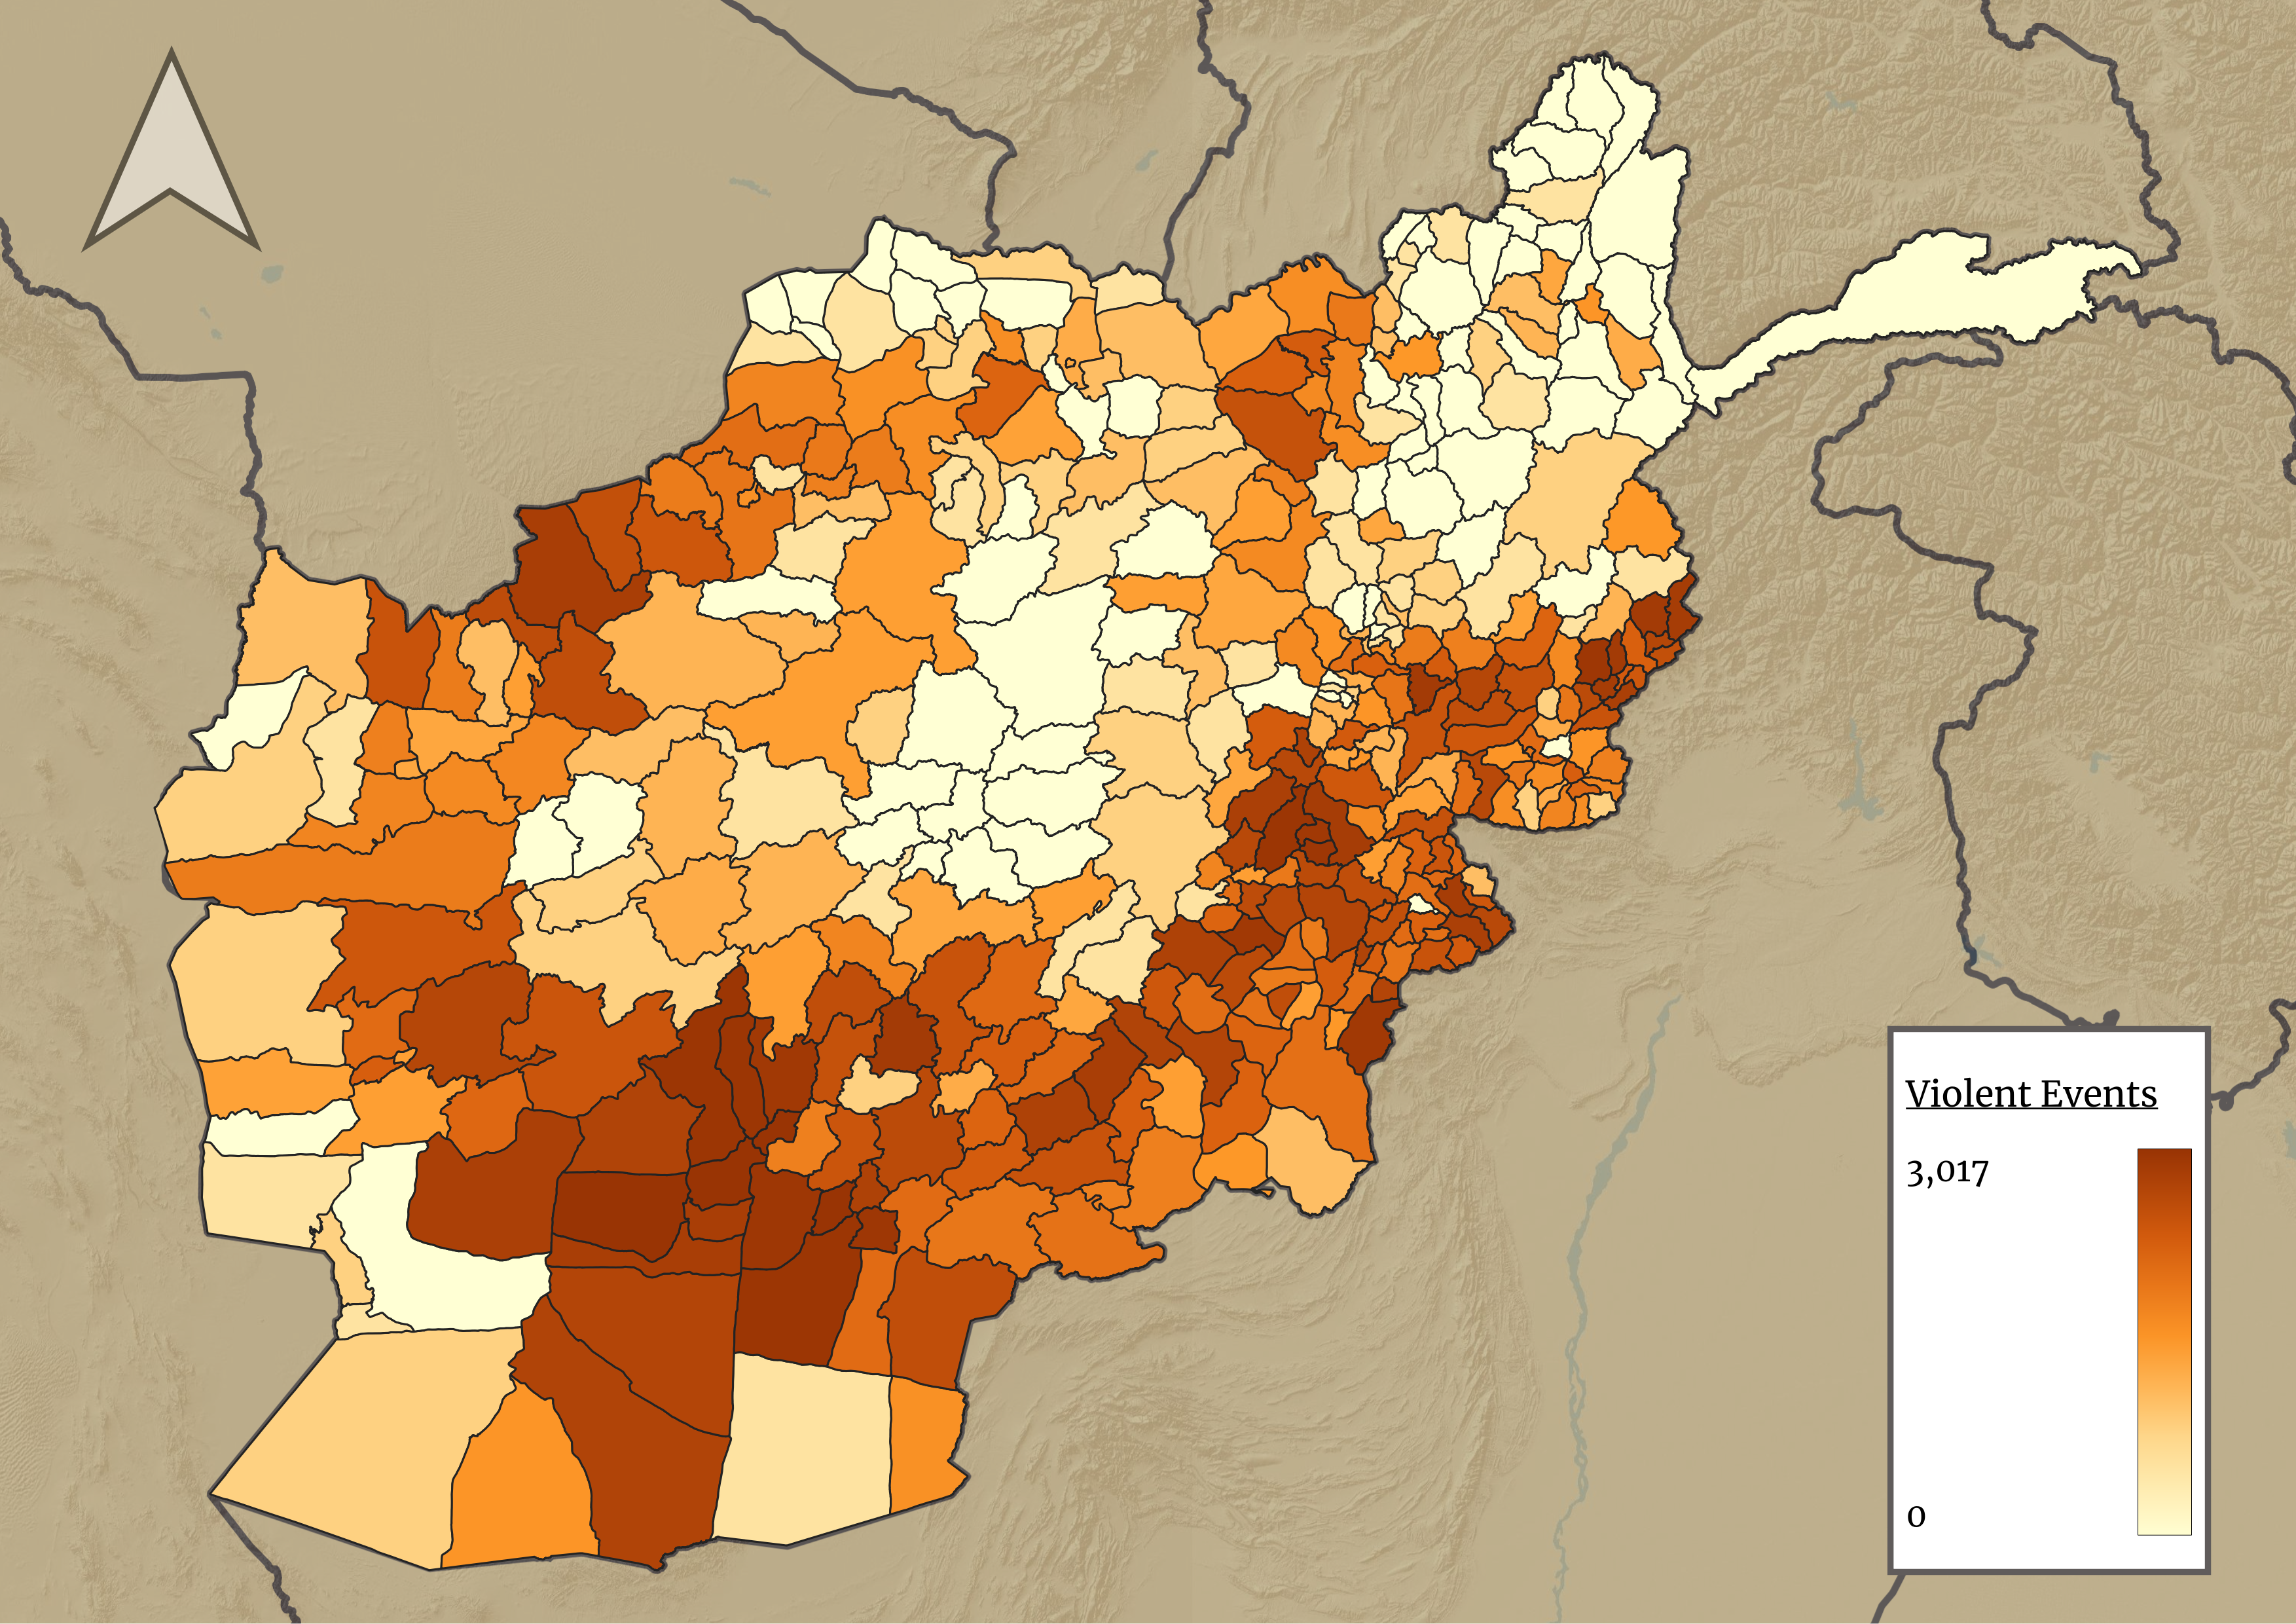
\includegraphics[width=0.8\linewidth]{analysis/results/figures/SIGACTS_events.png}
    \label{fig:sigacts_by_district}
    \vspace{0.25cm}
    \caption*{\small \textit{Notes:} Darker shaded districts experience more violence than lighter ones. Though SIGACT data contains several event types, I define violent exposure to include only direct fire, indirect fire, successful IEDs, and surface-to-air strikes. Notably, the category only includes violence accomplished by the insurgency.}
\end{figure}

\noindent This project is primarily concerned with insurgent violence, but SIGACT does contain records of counterinsurgent actions and to a lesser extent, civilian crime. Figure \ref{fig:sigacts_actor} shows the relative frequency of activity in SIGACT by actor (insurgent, counterinsurgent, or civilian). For a breakdown of insurgent violence only, see Figure \ref{fig:sigacts_type}: a timeline of the four main insurgent attack types. Direct fire events are the most commonly recorded. Violence types with higher production costs are less common, and it is unclear how civilians might respond differently to seeing surface-to-air missiles, improvised explosives, or mortar shelling, as opposed to gunfire. For simplicity in the main analysis, I group all insurgent actions together as a total violence indicator. 


\begin{figure}[h]
    \centering
    \caption{Total SIGACTs by actor during sample period}
    \includegraphics[width=0.8\linewidth]{analysis/results/figures/sigacts_actor.png}
    \vspace{0.25cm}
    \caption*{\small \textit{Notes:} This graph compares all SIGACTs by actor, without the author's specified violence categorization. Insurgent actions therefore include threats, found and cleared IEDs, and all the categories shown in Figure \ref{fig:sigacts_type}. Crime is committed by non-combatant civilians.}
    \label{fig:sigacts_actor}
\end{figure}

\begin{figure}[h]
    \centering
    \caption{Insurgent violence by type during sample period}
    \includegraphics[width=0.8\linewidth]{analysis/results/figures/sigacts_type.png}
    \vspace{0.25cm}
    \caption*{\small \textit{Notes:} Though SIGACT data contains several event types, I define a binary variable for violent exposures that includes only direct fire, indirect fire, successful IEDs, and surface-to-air strikes. Each of these describe acts of violence accomplished by insurgent actors only.}
    \label{fig:sigacts_type}
\end{figure}


\subsection{Call detail records (CDR)}

The SIGACT event records are spatially and temporally merged to a set of call detail records (CDR) from the largest Afghan cellular service provider, Roshan. Specifically, the records are from subscribers to Roshan's mobile banking service, M-Paisa. The data are provided in a user-by-day panel, allowing clustering for statistical inference at the individual level. The 17-month panel of over 15,000 users gives just under 3.5 million observations. Importantly, users do not enter or exit the sample in a uniform pattern.\par
Of course, there is selection into cell phone ownership, and again into mobile-banking, both of which could hamper the external validity of the study. In 2011, 46\% of all Afghans had a cell phone, and 9\% had a mobile bank account \citep{world_bank_world_2015}. However, there are reasons to assume a high level of variation among M-Paisa users, even if the sample may not perfectly represent the population as a whole. One might expect an outsized portion of the mobile banking users to be wealthy early adopters of new technology. In fact, the M-Paisa rollout included contracts with varied groups such as the Afghan National Police, Roshan's employees, and humanitarian groups that distribute cash aid \citep{blumenstock_violence_2024}. Even with promising variation in user type, the conclusions of this paper should be understood to be susceptible to some amount of selection bias. However, because the call detail records are anonymous and contain no additional user traits, the likely direction and magnitude of the bias is ambiguous. This is a common limitation of digital trace data like call records or social media posts, where data are generated by normal use of a consumer product. As the penetration rate of the product increases in a given research setting, digital trace data become more fully representative.\par 
Call detail records are unique among big data types. Unlike a geotagged Facebook post, which utilizes a phone's GPS system, the latitude and longitude reported by CDR data are not the exact location of a user at a given time. Instead, these data are records of calls, texts, or transaction activities matched to the location of the cell tower that transmits the corresponding signal. The user's location is inferred with various measures of centrality, discussed below. The number and locations of towers is thus vital in understanding the accuracy with which call detail records map to reality. By 2011, cell towers were ubiquitous in all populated areas of Afghanistan. Their distribution is not random, but they provide a level of fine granularity acceptable for large sample generalizations \citep{blumenstock_inferring_2012,chi_general_2020}. As shown in Figure \ref{fig:towers}, cell towers in Afghanistan map onto population centers. The general ring shape of the distribution of cell towers closely follows the highway system linking major cities. In the aggregated panel used for this study, tower coordinates corresponding to each phone use event are averaged over a 1-day period, reported as a daily center of gravity (COG). That is, for cell phone user $i$, who makes or receives $K$ calls on day $t$, define her daily center of gravity as,
\begin{equation}
     \frac{1}{K}\  \sum_{k=1}^{K} r_{itk} \
\end{equation}
where $r_{itk}$ is the vector of latitude and longitude coordinates, $\binom{lat}{lon}$, associated with the tower location of each call $k$. Thus, each user in the data has exactly one observation per day in sample, and the associated coordinates represent an average location derived from the nearest towers. In the available data, days with no usage are imputed with the previous day's COG. See Appendix \ref{app:A} for further discussion of imputation in the sample, including statistics.\footnote{The work of collapsing M-Paisa data to daily averages, COG imputations, as well as the merger with SIGACT events, was done upstream of this research use case. See \cite{blumenstock_violence_2024} for more information on the data.} I create several versions of the data, subject to restrictions on imputations, and find that results are largely consistent. That said, I drop individuals with a total time in sample less than 31 days, as my preferred definitions of migration events require at least one consecutive month of residency to establish the home location from which one could migrate.\\

\begin{figure}[h]
    \centering
    \caption{Roshan cell towers in Afghanistan, 2011}
    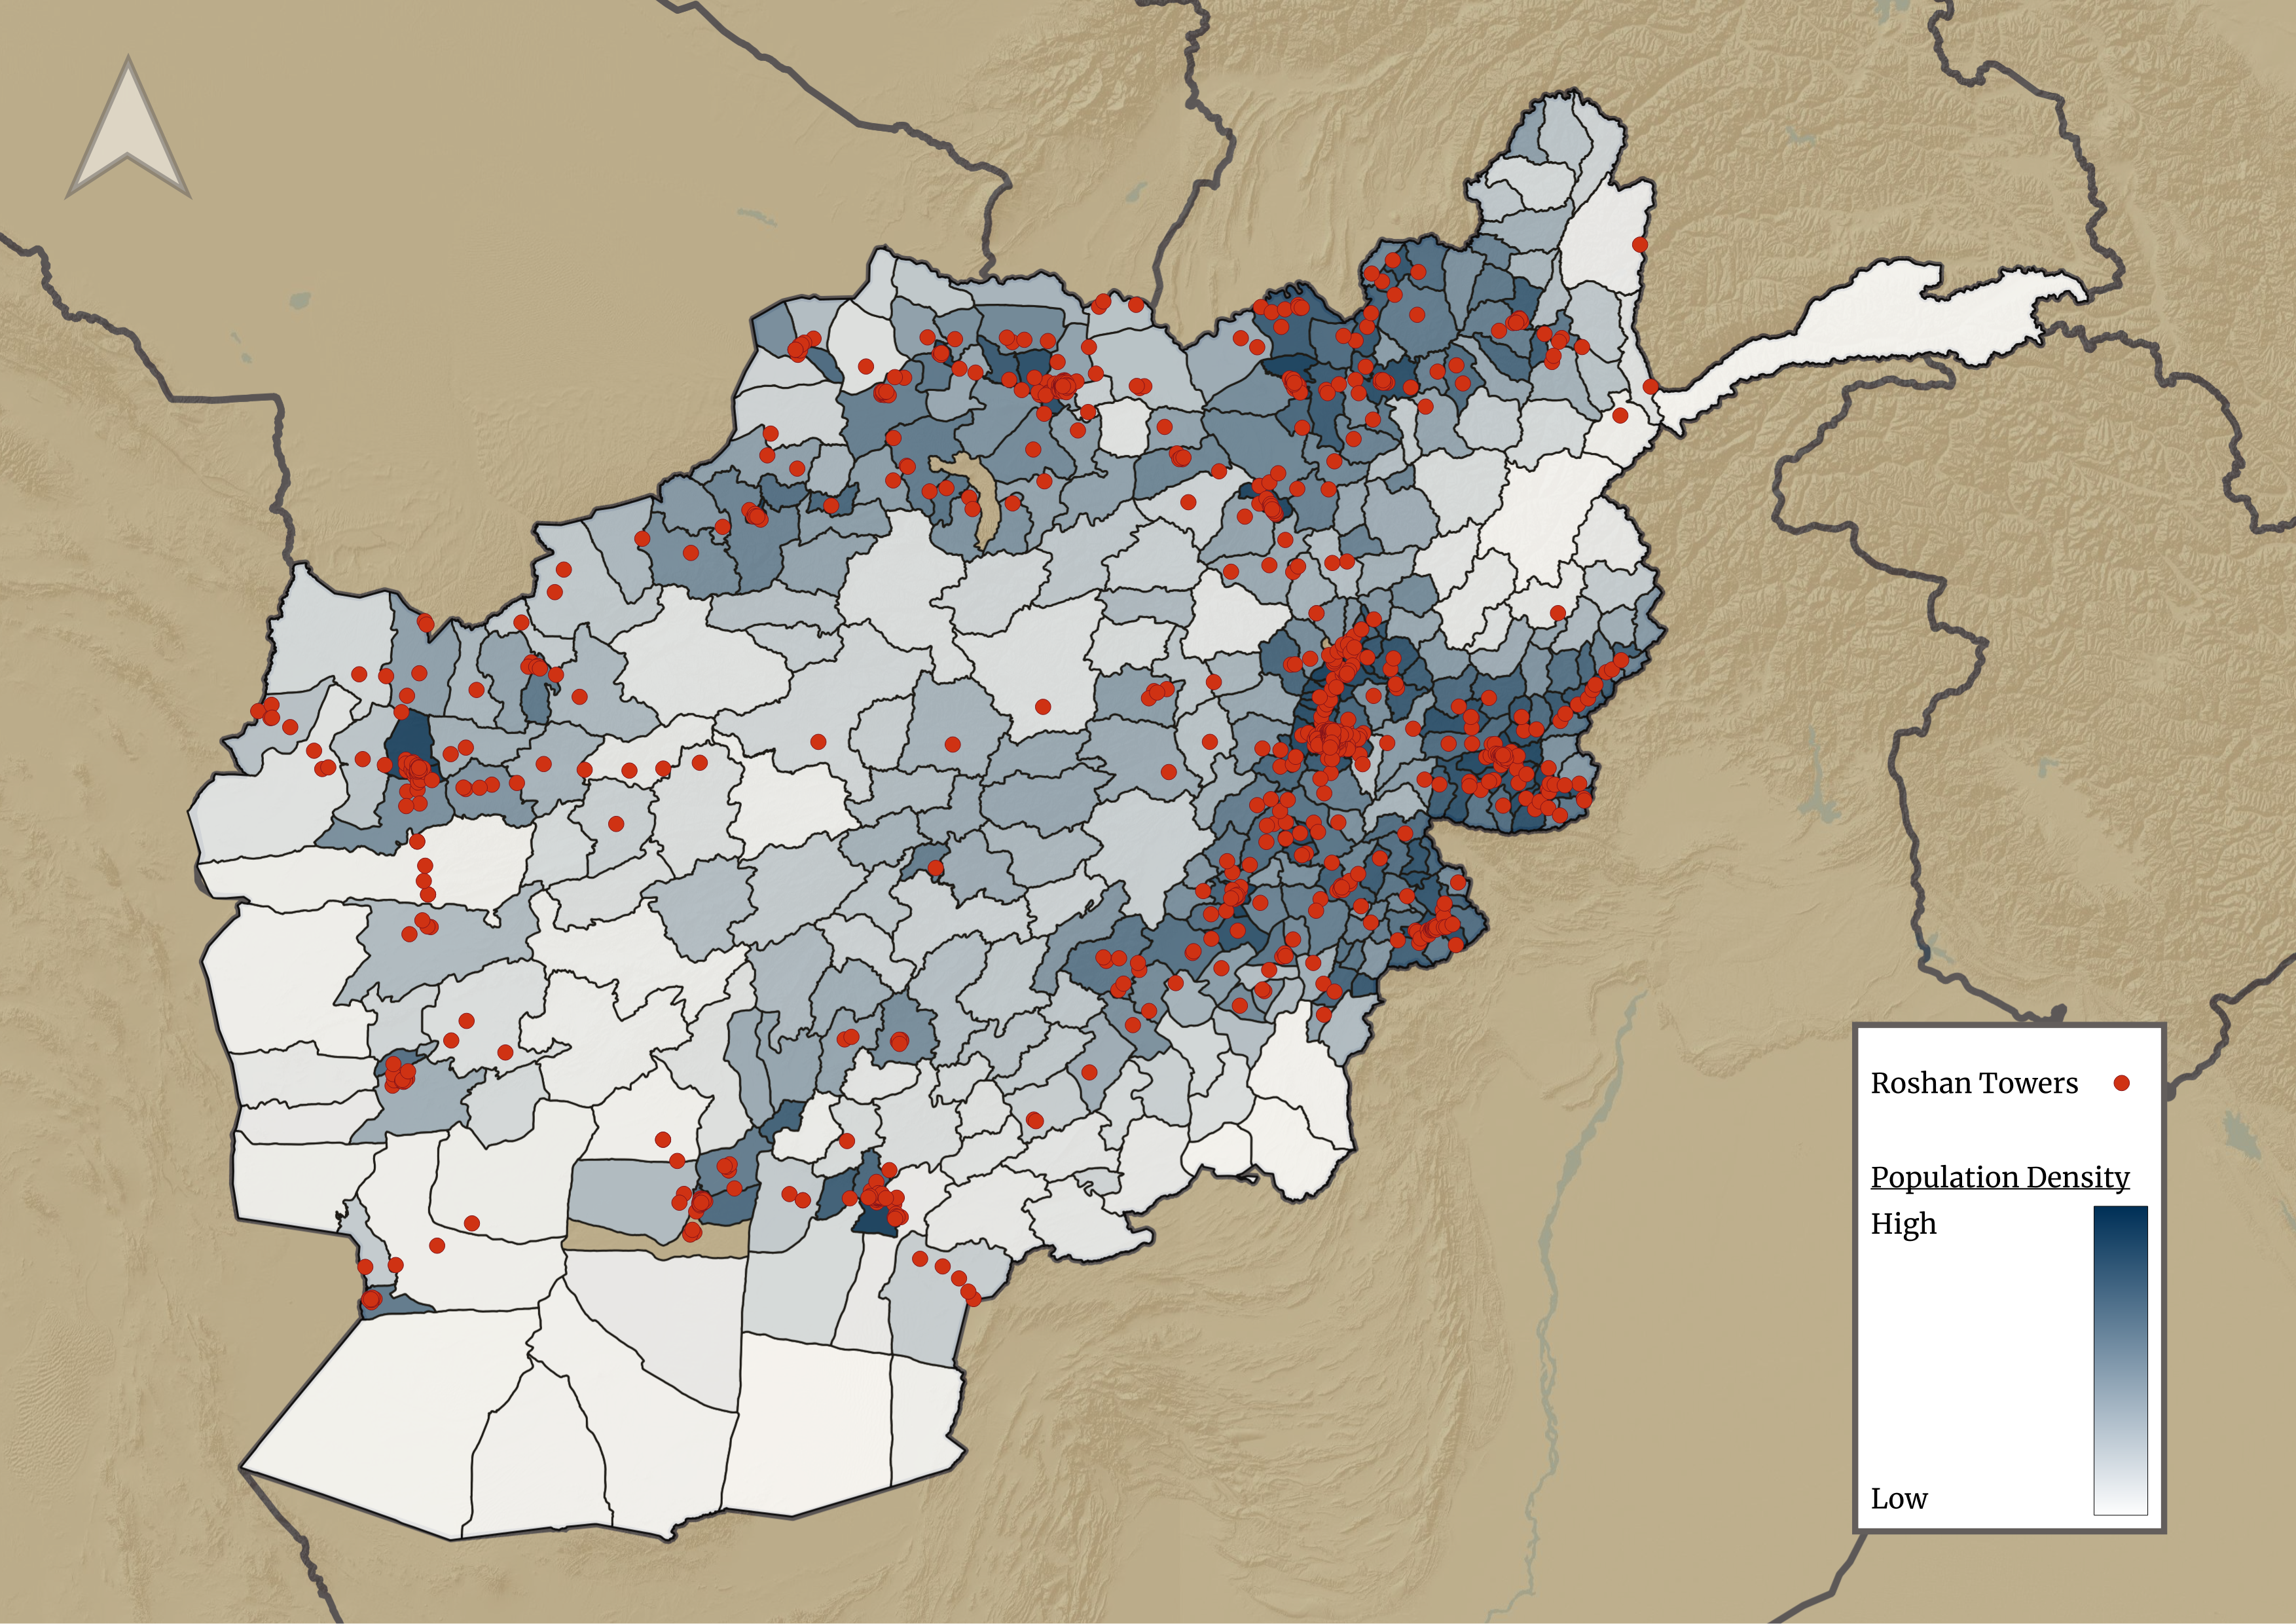
\includegraphics[width=0.8\textwidth]{analysis/results/figures/afg_roshan_popdensity.png}
    \vspace{0.25cm}
    \caption*{\small \textit{Notes:} Red dots denote cell tower locations, which were obtained from Roshan. Population density was obtained from \cite{ciesin_-_columbia_university_gridded_2016}. Shading shows density at the district level, with high-density areas in darker blue.}
    \label{fig:towers}
\end{figure}

\subsection{Measurement}

The M-Paisa call detail records are merged at the daily level with SIGACT violent events. For user $i$ at time $t$, define a binary exposure variable $D^{\rho}_{it}$ equal to one (1) if her daily COG was within some radius $\rho$ of a SIGACT event. In this study, $\rho$ takes on only the discrete values of 5 and 20 kilometers. $D^{\rho}_{it}$ can also be broken into attack types, e.g. direct fire, indirect fire, or IED attack. I find that most specifications provide consistent results across attack types, and for simplicity use an indicator that includes all of them. From $D^{\rho}_{it}$, I construct a count-style variable, as users in areas with high target-value can be exposed to multiple events per day. I then normalize the count of exposures by a measure of time to simplify interpretation of regression results. Table \ref{tab:sumstat} describes the high frequency of violent exposure in this setting. 89\% of M-Paisa users are exposed within 5km to at least one insurgent event during the sample period. On average, users are exposed 0.06 times per day, approximately twice per month. Figure \ref{fig:cdr} provides an illustration of how SIGACT events are matched to daily centers of gravity to form the exposure variable.\\


\begin{table}[h]
    \centering
    \caption{5km exposures to violence, by individual user}       \begin{tabular}{l*{1}{cccc}}
\toprule
                &     Mean&       SD&      Med&      Max\\
\midrule
\vspace{0.1em} \\ \emph{Panel A: Violence (Ever exposed)}&         &         &         &         \\
\hspace{0.25cm} All violence&     0.89&     0.31&     1.00&        1\\
\hspace{0.25cm} Direct fire&     0.80&     0.40&     1.00&        1\\
\hspace{0.25cm} Indirect fire&     0.39&     0.49&     0.00&        1\\
\hspace{0.25cm} Surface-air&     0.48&     0.50&     0.00&        1\\
\hspace{0.25cm} IED&     0.75&     0.43&     1.00&        1\\
\vspace{0.1em} \\ \emph{Panel B: Violence (Total exposures)}&         &         &         &         \\
\hspace{0.25cm} All violence&    13.84&    27.66&     6.00&      399\\
\hspace{0.25cm} Direct fire&     6.15&    16.57&     2.00&      305\\
\hspace{0.25cm} Indirect fire&     1.48&     3.35&     0.00&       47\\
\hspace{0.25cm} Surface-air&     1.14&     1.69&     0.00&       19\\
\hspace{0.25cm} IED&     5.06&    10.50&     2.00&      106\\
\vspace{0.1em} \\ \emph{Panel C: Violence (Per day)}&         &         &         &         \\
\hspace{0.25cm} All violence&     0.06&     0.09&     0.04&        2\\
\hspace{0.25cm} Direct fire&     0.03&     0.06&     0.01&        1\\
\hspace{0.25cm} Indirect fire&     0.01&     0.01&     0.00&        0\\
\hspace{0.25cm} Surface-air&     0.01&     0.01&     0.00&        0\\
\hspace{0.25cm} IED&     0.02&     0.03&     0.01&        1\\
\bottomrule
\end{tabular}

    \label{tab:sumstat}
    \vspace{.25cm}
    \caption*{\small \textit{Notes:} Excludes data from imputation gaps. Data are collapsed to the individual user-level. For restricted samples that further limit the number of imputed observations, see Appendix \ref{app:A}. For the same statistics for 20km exposures to violence, see Table \ref{tab:sumstat_20km} in Appendix \ref{app:B}.}
\end{table}

\clearpage


\begin{figure}[h]
    \centering
    \caption{Identifying exposure to violent events}
    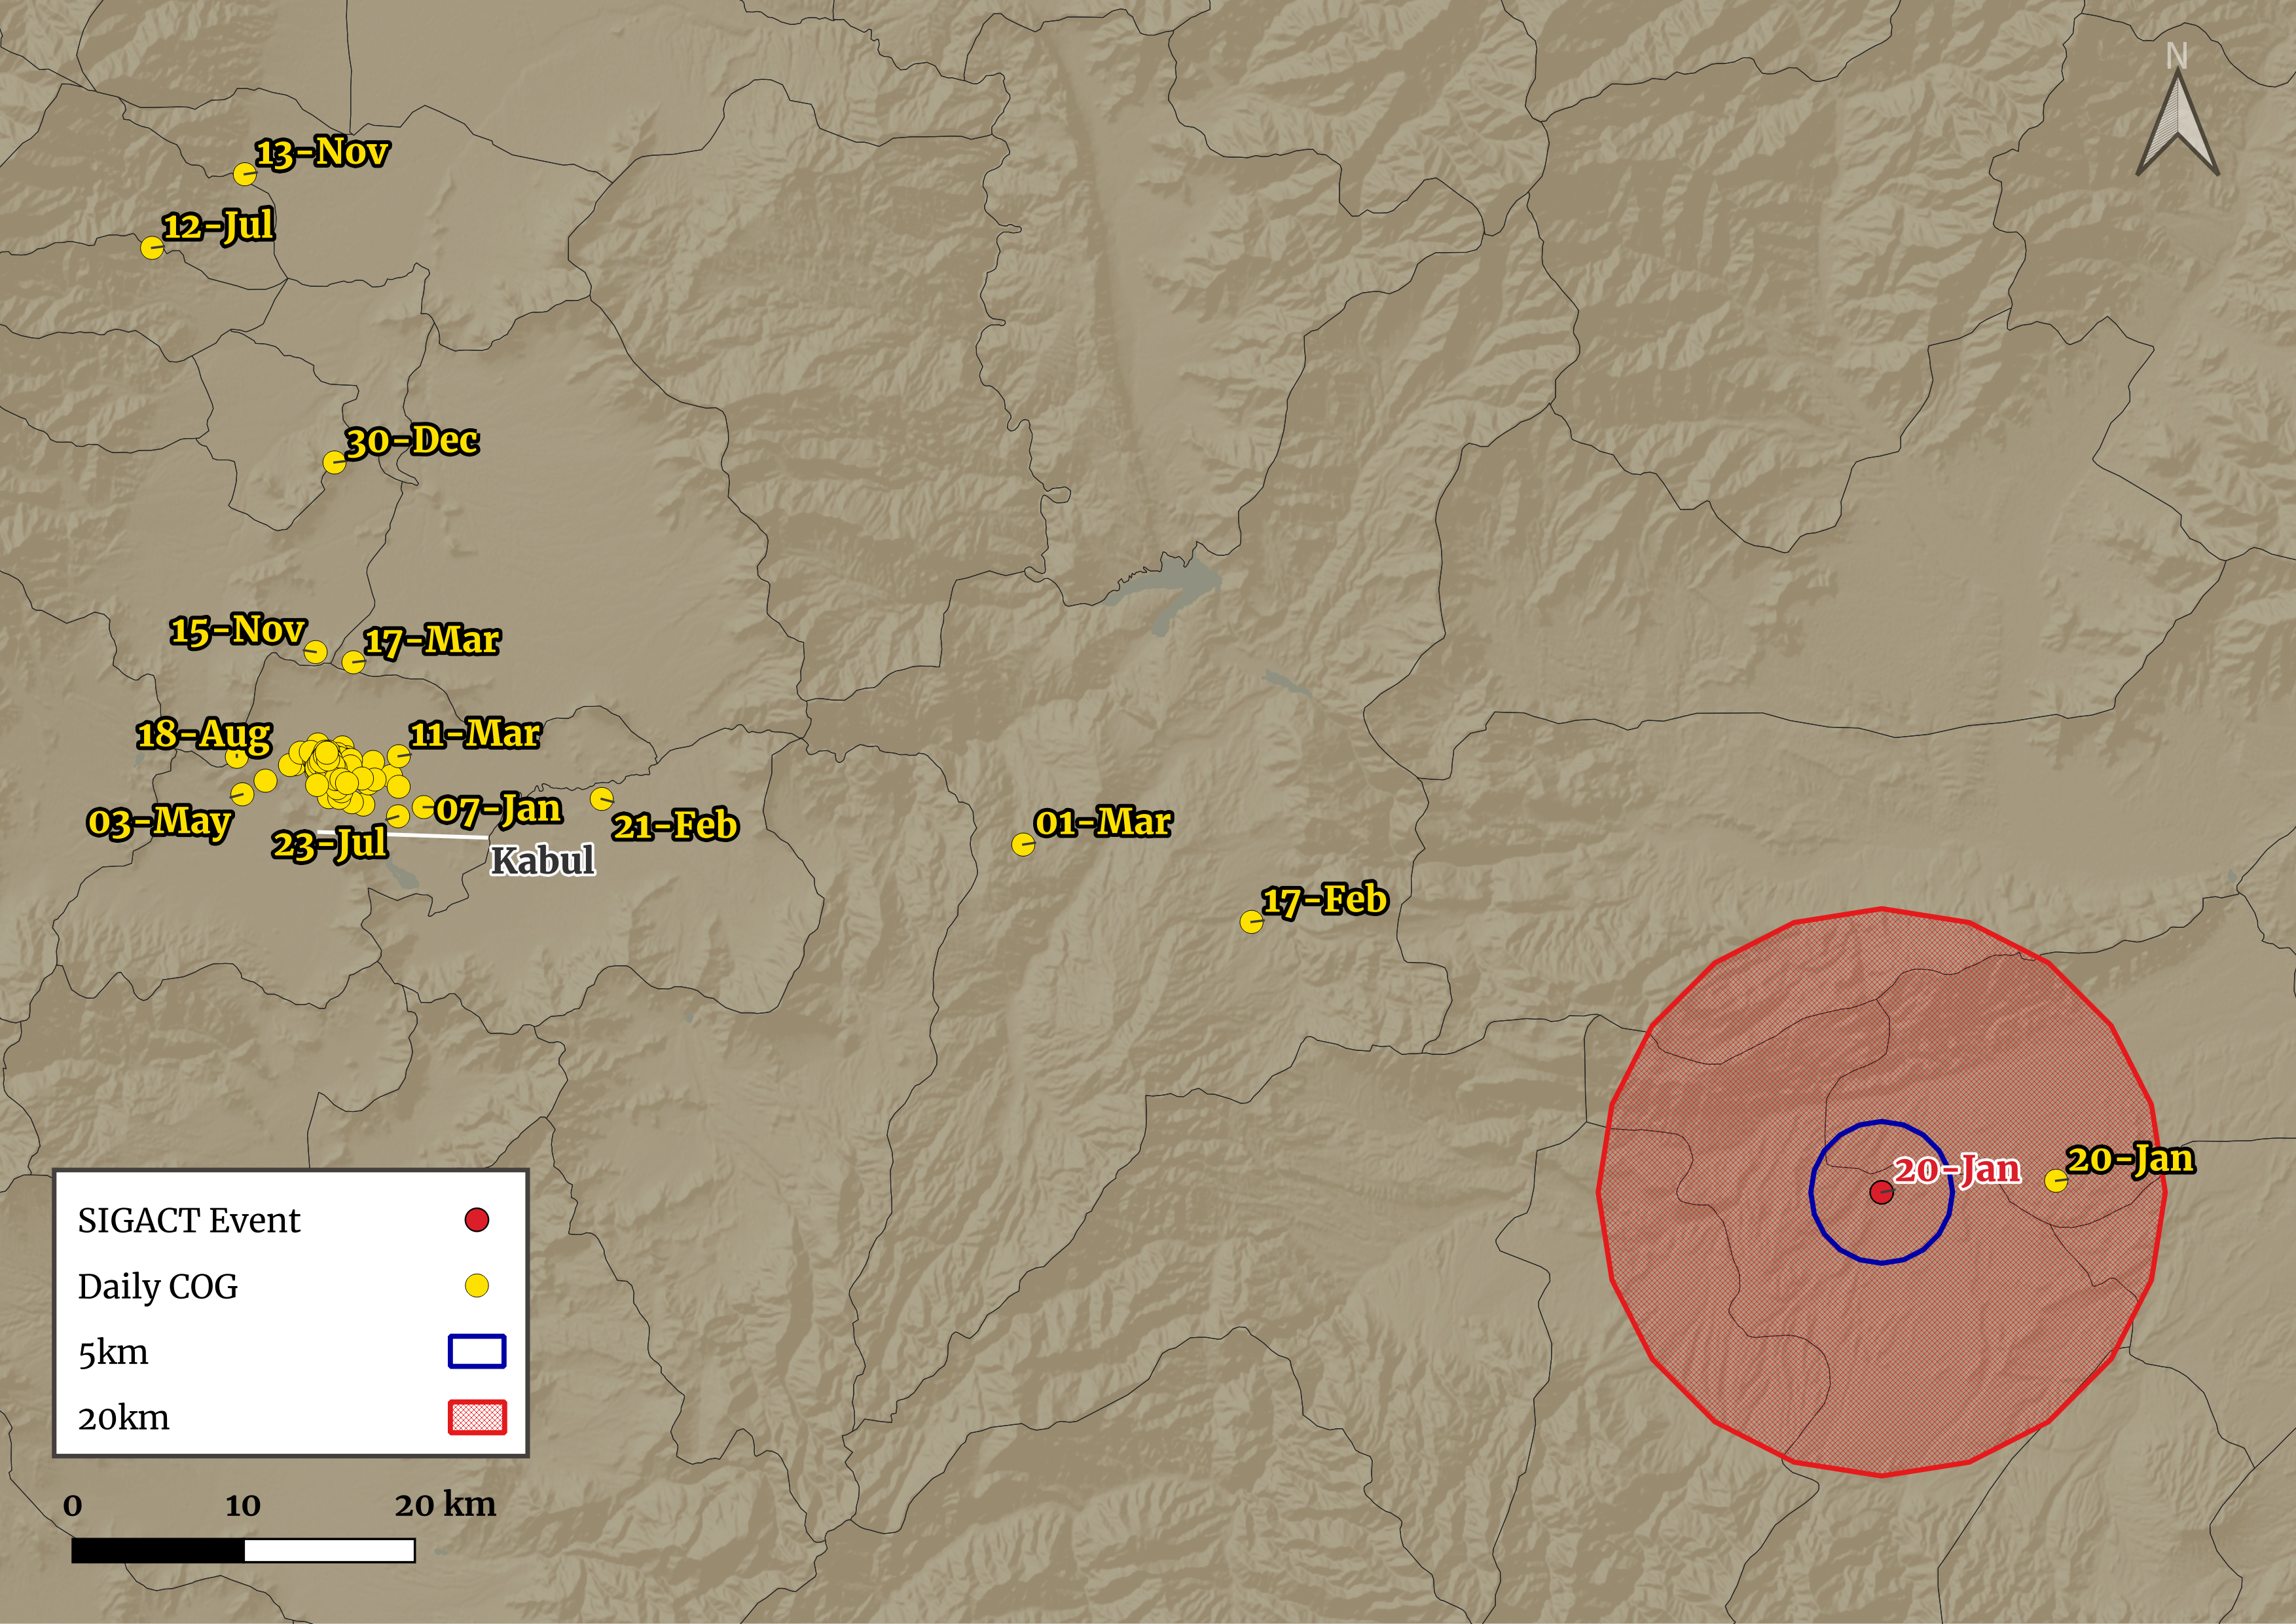
\includegraphics[width=0.9\textwidth]{analysis/results/figures/cog_example_jmp.png}
    \vspace{0.25cm}
    \caption*{\small \textit{Notes:} Yellow dots show the set of locations for a randomly-selected Roshan user. The red dot represents a violent event from SIGACT. The location of the red dot is for illustrative purposes only, and does not represent an actual event from the data. A single yellow dot sits inside the red circle, which represents a 20km radius from the hypothetical event. Notice, the date of the violent event must match that of the user-location observation within its exposure range. This user-day observation would receive a $1$ for the binary variable indicating a 20km exposure. As illustrated by the blue circle, that same user-day observation would be coded $0$ for the variable indicating a 5km exposure.}
    \label{fig:cdr}
\end{figure}

\noindent One strength of CDR is their precision. As given, the coordinates have a resolution of about one square meter. Researchers have noted that in areas with a high density of cell towers, movements can be falsely recorded among nearby towers \citep{milliff_big-data_2022}. To account for this, I coarsen the data to a resolution of about one square kilometer to capture changes in centers of gravity that are appropriately distant from one another for the measurement of migration events. The result is similar to imposing a grid of 1km cells over the area of the country to track discrete user locations. I follow \cite{blumenstock_inferring_2012} and others, coding each user's monthly modal location as their home center of gravity. Results do not differ substantially with other denominations of home, such as monthly mean location. I encode a unique value to each ordered lat-lon pair visited in the entire dataset, and calculate the modal pair for each user, every month they are in the sample. I then calculate distances (km) between users' daily COG and home location \citep{picard_geodist_2019}. Even though the observation is technically an average of tower locations, I refer to it as the \textit{user's} COG for simplicity. Other variables are generated from the distances and coordinates, such as a binary indicator for being outside one's home district or province. Another variable, the user's \textit{radius of gyration} (ROG), is a statistic constructed to represent the geographic extent of one's movements over time. The ROG is the root mean square distance of all locations a user visits from their home center of gravity.


\section{Classifying cross-border migration events} \label{sec:method}
\subsection{Motivation}

Researchers using administrative or survey data at the individual or household level are rarely able to identify migrants themselves, for the simple fact that most countries' statistical agencies collect data only within their national borders. Consider an individual from country $A$ who migrates to country $B$. They might be present in data collected by $A$ up until the date of migration, but as a resident of $A$ only. Their status as a migrant is a future development; it is concurrent with their disappearance from the data $A$ collects. Once in country $B$, the same individual could be identified as a migrant in a census or survey within $B$, but often with little to no information about their life before arrival. A researcher interested in the determinants of migration (or the welfare of migrants in their host countries) would prefer individual or household data with information from both $A$ and $B$. While many host countries do identify noncitizens in their statistical records, there is rarely enough additional information to meaningfully link individuals to anything more than their country of origin. The American Community Survey, for example, collects data on foreign-born residents, but only identifies one's place-of-origin from among six continental regions. This project is the first to use CDR data to infer international migrations. Subsequently, the method provides a potential solution to the data problem described above, allowing researchers to observe both migration events and pre-migration histories at the individual level. This is especially useful in settings like Afghanistan where the last government census was collected in 1979. While researchers do conduct surveys in Afghanistan, I am aware of none that attempt to measure out-migration from interviews at border crossings or airports, or by other means.\footnote{The 2011 Afghanistan National Risk and Vulnerability Survey contains a question about the migration of family members.}

\subsection{General method}

There are several challenges to inferring international migration from call detail records. I propose a method based on identifying attrition events that satisfy certain filtering restrictions, described below. Roshan does not record phone activity outside of Afghanistan, so one plausible reason for user attrition is that they have left the country by crossing a land border.\footnote{Even if a mobile network operator provides service on both sides of an international border, the networks themselves are bounded and discontinuous. When a user crosses the border with continuous service, this is accomplish by roaming; they drop from the origin country records no matter what.} Of course, there are many reasons why a user's activity could disappear from the data. I argue that most or all of these concerns are assuaged by the conditions that follow. In other words, each of the following restrictions serves to decrease the likelihood that an attrition event is due to reasons other than the user crossing an international border.\footnote{Some possiblities include nonpayment of the phone bill, canceling of the contract, or destruction of the phone or SIM card.}\par

Let $r_{iT} $ represent a user's location on their final day in the sample. I label user $i$ an external migrant if the following conditions hold:
\begin{equation} \label{eq:criteria1}
    (r_{iT} - COG^h_{iT}) \, > \, \delta * ROG_i
\end{equation}
\begin{equation} \label{eq:criteria2}
    (r_{iT} - r_{cross}) \, < \, \gamma
\end{equation}
\begin{equation} \label{eq:criteria3}
    T_i \, < \, T-\epsilon
\end{equation}
\begin{equation} \label{eq:criteria4}
    \frac{1}{S}\sum_{s=T_i-S}^{T_i} \biggl[ (r_{i,s+1} - r_{cross}) - (r_{is} - r_{cross}) \biggr] < 0
\end{equation}

\noindent where $COG^h_{iT}$ is the user's home location in the month of their attrition, $\delta$ is a flexible scaling parameter, and $ROG_{i}$ is the user's average radius of gyration. The inclusion of $ROG_{i}$ accounts for differences in typical mobility across individuals. This condition simply requires a user be suitably far from home, moderated by the limits of their average movement. In equation \ref{eq:criteria2}, $r_{cross}$ is the location of a known border crossing (see Figure \ref{fig:boundary}), and $\gamma$ is a flexible distance parameter. This condition requires a user be sufficiently near a border crossing point before attrition. In (\ref{eq:criteria3}), $T_i$ is the date of the user's final day in the sample, $T$ is the full sample final date, and $\epsilon$ is a flexible time parameter. This condition removes the possibility that an attrition event is simply due to the end of the sample. Finally, in (\ref{eq:criteria4}), I define $s\in{S}$ to be a set of lead-up days before attrition. Since each user is closest to a single $r_{cross}$ on their final sample day, I trace their movement toward the border crossing over $S$ days, requiring that on average they move toward it, rather than away. This filters remaining individuals who may simply live near a border crossing, or those who have extended periods of non-usage leading up to attrition. To summarize, these conditions imply the following: in order to be classified as an external migrant, a user must be a certain distance from home on their final day in sample, and simultaneously near a known border crossing. Additionally, I disqualify users whose final day is one of the last $T - \epsilon$ sample dates, i.e. they are not dropping out simply because they recorded no phone usage in the final $\epsilon$ days of total sample time. The condition described in equation (\ref{eq:criteria4}) stipulates that users' day-over-day distance to a final border crossing point is decreasing in the $S$ days leading up to their attrition from the data. Table \ref{tab:sumstat_mig} summarizes mobility and migration outcomes in the Roshan sample, and introduces two classifications of external migrant based on the tuning parameters in the classification scheme above. Internal migrations are identified using the method described in \cite{blumenstock_migration_2023}, whereby users' home locations change to one in another province for at least one month.\\


\begin{table}[H]
    \centering
    \caption{Migration statistics, by individual user}
    \begin{tabular}{l*{1}{cccc}}
\toprule
                &     Mean&       SD&      Med&      Max\\
\midrule
\vspace{0.1em} \\ \emph{Panel A: Mobility}&         &         &         &         \\
\hspace{0.25cm} Km from home&    10.91&    23.48&     3.02&      378\\
\hspace{0.25cm} Radius of gyration (km)&    19.09&    37.06&     5.73&      500\\
\hspace{0.25cm} Outside home district&     0.11&     0.14&     0.05&        1\\
\hspace{0.25cm} Outside home province&     0.04&     0.08&     0.00&        1\\
\vspace{0.1em} \\ \emph{Panel B: Migration}&         &         &         &         \\
\hspace{0.25cm} Internal migrant&     0.07&     0.25&     0.00&        1\\
\hspace{0.25cm} External migrant (1)&     0.03&     0.16&     0.00&        1\\
\hspace{0.25cm} External migrant (2)&     0.01&     0.08&     0.00&        1\\
\bottomrule
\end{tabular}

    \label{tab:sumstat_mig}
    \vspace{.25cm}
    \caption*{\small \textit{Notes:} ``Km from home'' is measured daily. Radius of gyration is a monthly statistic. Variables for ``outside home district'' and ``outside home province'' are binary and measured daily. Internal migrations are classified as in \cite{blumenstock_migration_2023}. The two types of external migrations represent a (1) lenient and (2) restrictive set of parameters, respectively. Excludes data from imputation gaps. Data are collapsed to the individual user-level. For restricted samples that further limit the number of imputed observations, see Appendix \ref{app:A}.}
\end{table}

\noindent There is substantial researcher choice in setting the tuning parameters of the classification criteria. As a bounding exercise, I choose the following parameter values under two different specifications, one lenient and one restrictive (see Equations \ref{eq:criteria1} - \ref{eq:criteria4}). For the \textit{lenient} classification of a migrant,
\begin{equation} \label{eq:lenient}
    \delta = 0.1 \ , \ \gamma = 75km 
\end{equation}
and the \textit{restrictive} classification,
\begin{equation} \label{eq:restrictive}
    \delta = 0.2 \ , \ \gamma = 50km 
\end{equation}

\noindent The chosen values of $\delta$ adjust the moderating effect of the radius of gyration ($ROG$) on the distance from home required for classification. The more restrictive model requires that individuals be further from home than the lenient model. The choice of $\gamma$ is particularly setting-specific; values too large risk falsely classifying those simply visiting population centers near border crossing points. I choose 75km in the lenient classification based on the nearness of Jalalabad to the Torkham border crossing. Researchers may also adjust the value of $\epsilon$; here it is set to 1 for both classifications.
% OBVIOUSLY WANT TO TALK MORE HERE ABOUT METHOD

\subsection{Limitations and validation}

The locations of Roshan towers in 2011 covered almost all of Afghanistan's population, but a slightly smaller proportion of its total land area. Because user centers of gravity are calculated from a daily average of tower locations, I only observe locations within the convex hull of Roshan towers intersected by the national borders of the country.\footnote{The boundary of the convex hull is the simple closed curve with minimum perimeter that contains all the towers.} As illustrated in Figure \ref{fig:boundary}, it is possible that users in the remote southwest of the country receiving service could appear in the data with inaccurate location measurement. However, as seen in Figure \ref{fig:towers}, population is very sparse in areas without coverage from Roshan. Another potential issue arising from Figure \ref{fig:boundary} is the fact that not all known border crossings fall within the coverage boundary. The white dots, especially those at the southern border, are mechanically left out of this analysis. However, the vast majority of all migration and commercial activity occurs in a relative few crossing points, specifically those shown with their names. All of these are fully within the coverage area.\par
The usefulness of the CDR attrition method to infer external migrations is limited by the data available to fully validate it. For example, GPS data do not suffer from the constraints of national borders, and thus offer the best potential validation for the classifying criteria. Obtaining GPS data are outside the scope of this project, but future research considering this method should seek to validate it in this way.\\


\begin{figure}[h!]
    \centering
    \caption{The intersection of Afghan borders and the convex hull of Roshan towers}  
    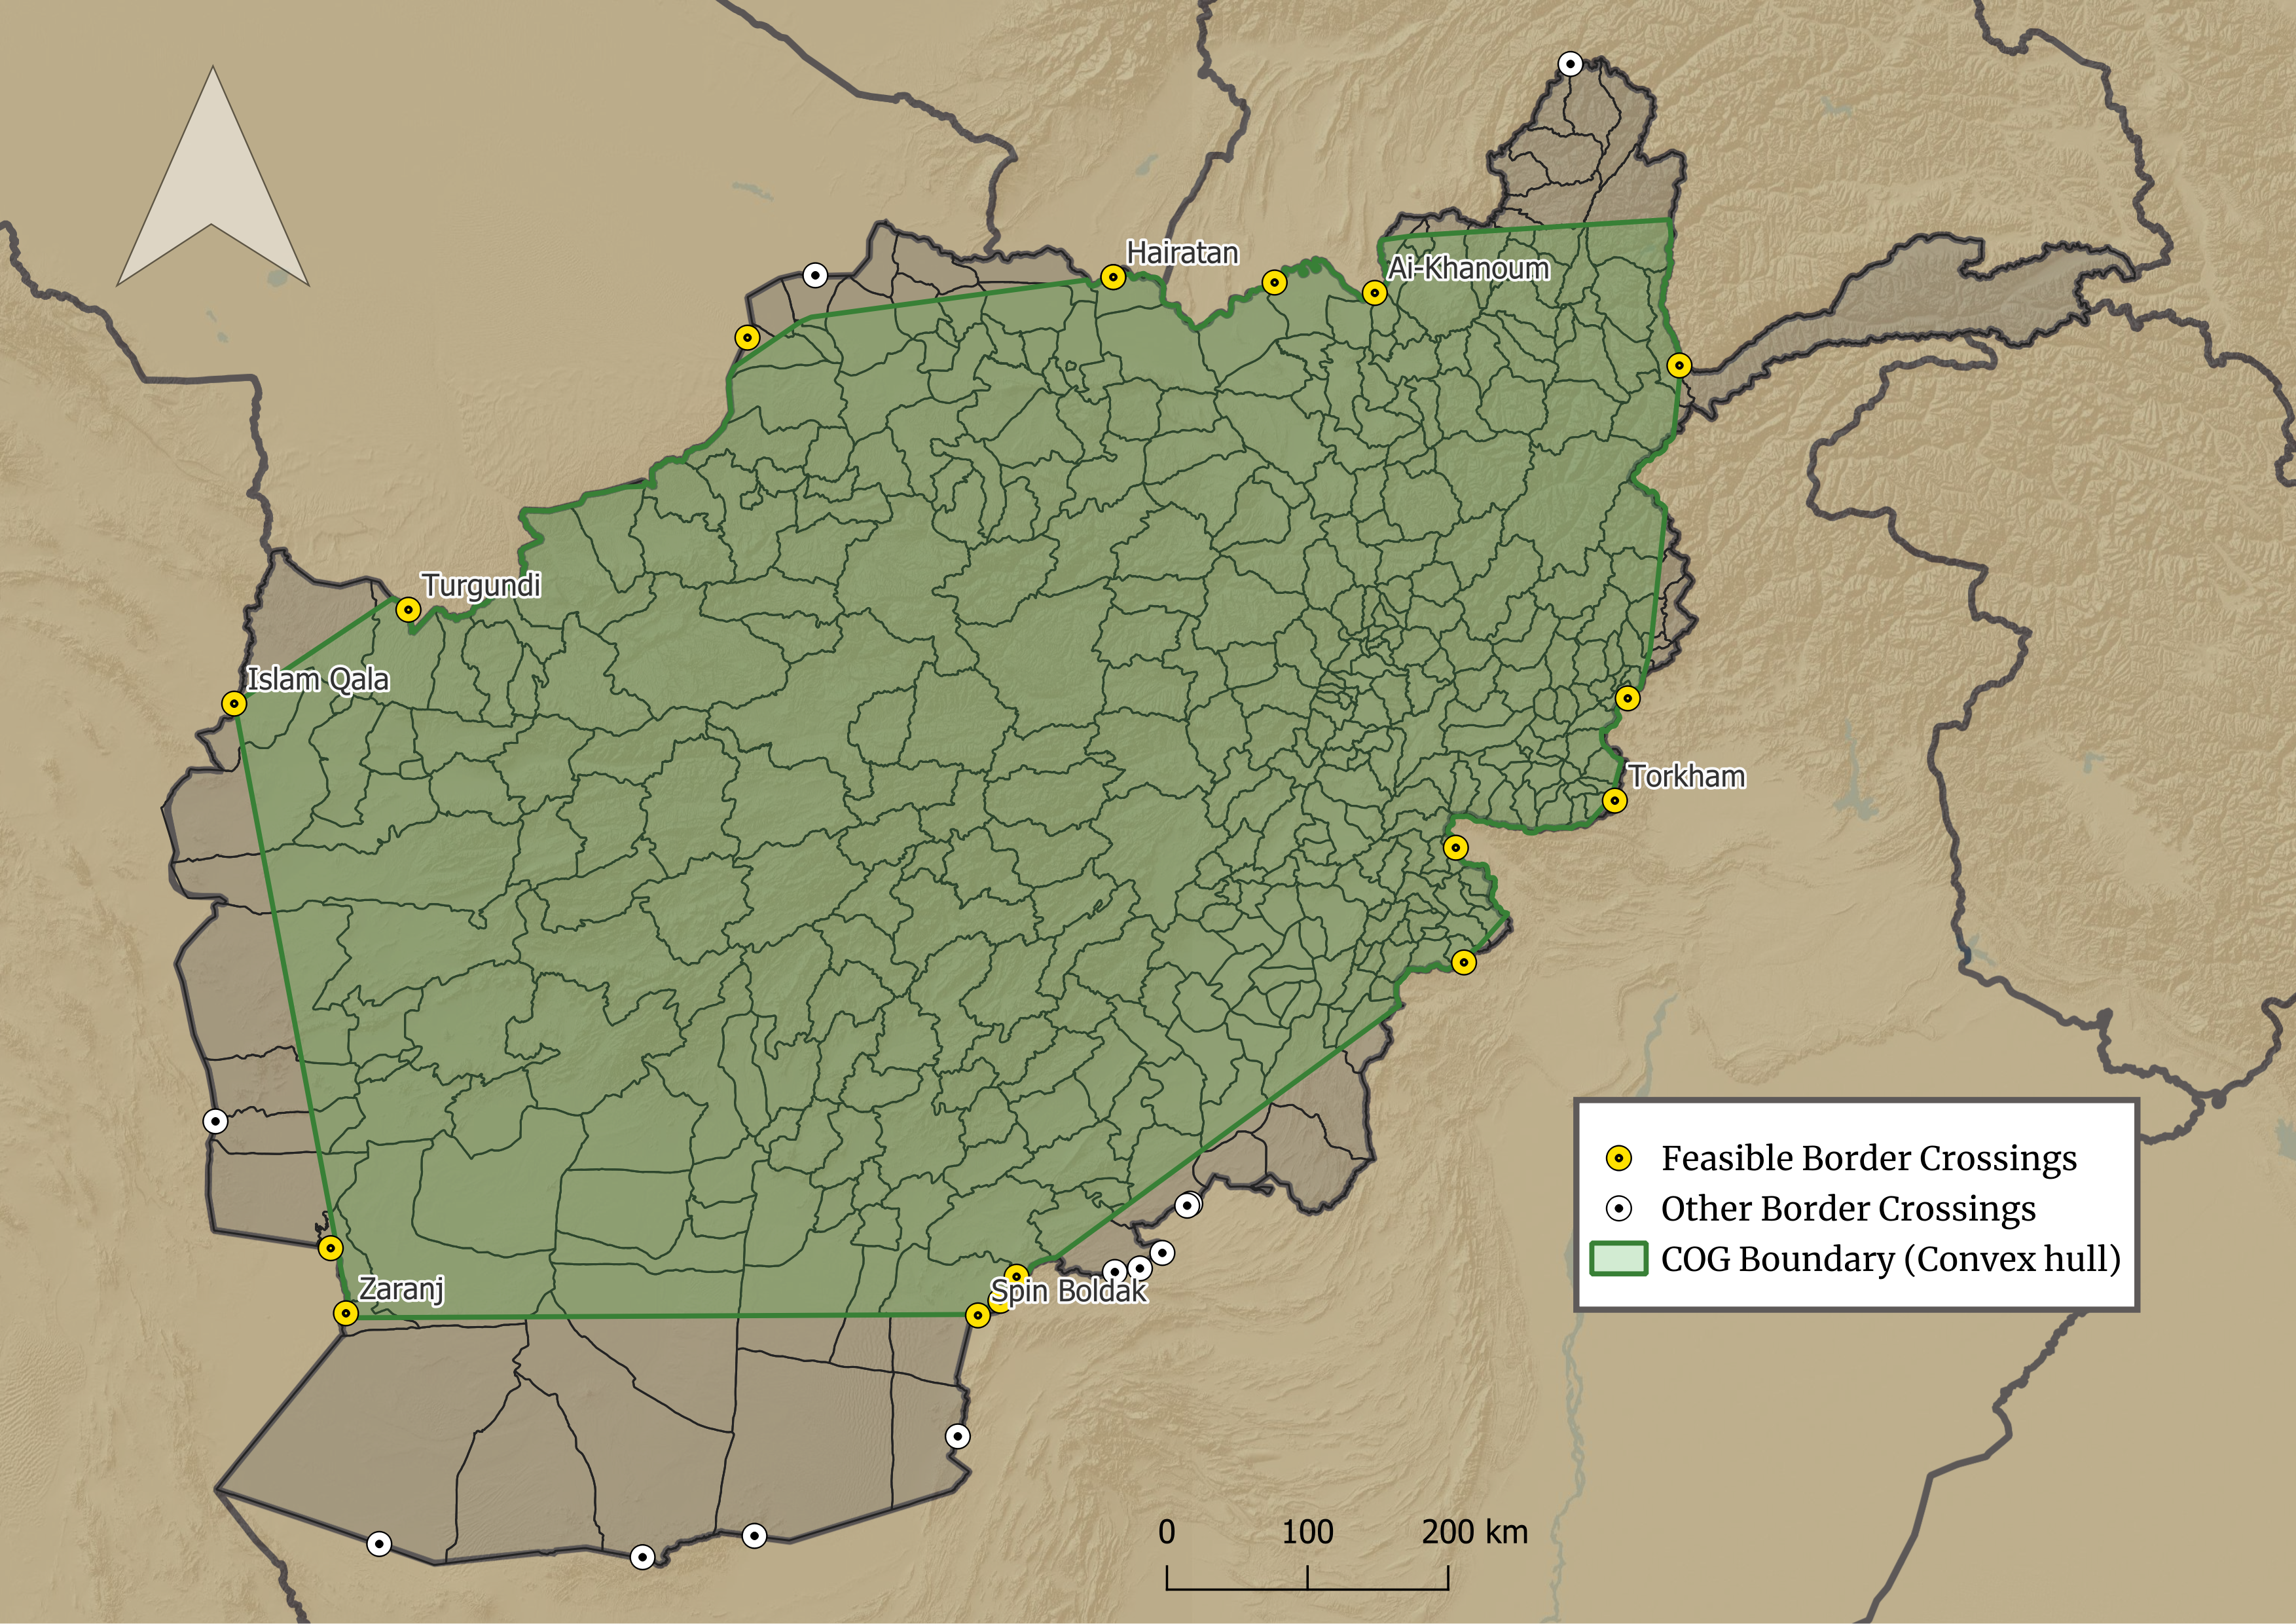
\includegraphics[width=0.8\linewidth]{analysis/results/figures/convex_hull.png}
    \vspace{0.25cm}
    \label{fig:boundary}
    \caption*{\small \textit{Notes:} The green shaded area is the convex hull of Roshan towers intersected with Afghanistan's national borders. This map illustrates the fact that even if an individual successfully uses their phone outside the green area, their location in the data will be coded as that of the nearest tower to them, on or near the boundary of the shaded region. Also present are known border crossing locations. Yellow dots are border crossings that are feasibly covered by the convex hull of tower locations, and white crossings are not. The external migration results do not change with the inclusion/exclusion of the crossings outside the shaded area.}
\end{figure}

%%%%%%%%%%%%%%%%%%%%%%%%%%%%%%%%%%%%%%%%%%%%%%%%%%
%%%%%%%%%%%%%%%%%%%%%%%%%%%%%%%%%%%%%%%%%%%%%%%%%%

\section{A model of displacement choice} \label{sec:model}
\subsection{Binary choice}

A simple model, adapted from \cite{ibanez_civil_2008} and \citep{chin_chapter_2015}, is useful to illustrate the individual migration decision. An individual decides to migrate (internally or internationally) based on an inequality in expected utility between their home and a receiving area. Define $P^M \equiv I(V_{id} - V_{ih})$ where $I(\cdot)$ is the index function, and indirect utility $V_i$ is indexed over a home location and a single destination location:

\begin{equation}
    V_{ih} = \alpha S_{ih} + \beta w_{ih} ,
\end{equation} 

\begin{equation}
    V_{id} = \alpha S_{id} + \beta(w_{id} - C_{ihd}) .
\end{equation}

\noindent Individual $i$ will migrate from home location $h$ to destination $d$ when $P^M>0$.  $w_{i}$ represents location-specific wages, $C_{ihd}$ are the migration costs from $h$ to $d$, and $S_{i}$ are individual perceptions of security, also unique to each location choice. First order conditions imply that utility is increasing in destination safety ($\frac{\partial P^M}{\partial S_{id}} > 0$), and thus a difference in $S_{id} - S_{ih}$ of sufficient magnitude could shift those on the margins into displacement. As expected, migration is decreasing in costs ($\frac{\partial P^M}{\partial C_{ihd}} < 0$) and home wages ($\frac{\partial P^M}{\partial w_{ih}} < 0$).\footnote{Migration choice models often combine amenities such as safety into the cost term, but in this context it is useful to make explicit the disutility of non-economic concepts like violence.}\par




%\subsection{Location choice}

%\textit{*Paragraph forthcoming: model extension to multiple locations*} \\

\section{Estimation and results} \label{sec:empirics}
\subsection{Simple and conditional logit} \label{simplelogit}

After identifying potential migration episodes via the methods described above, I estimate a cross-sectional logit regression. Though it cannot account for an expanded choice set, simple logit estimation is canonical in empirical migration work. In this paper, it is useful in identifying the extensive margin of international migration choice. In this specification, I identify the change in a users' odds of migrating in response to an increase in their monthly rate of violent exposures, conditional on individual and geographic controls.\footnote{Perhaps more accurately, these are the odds of classifying a user as a potential migrant with the criteria developed in this paper. Controls include mean ROG, days present in sample, and home province indicators.} In Table \ref{tab:simplelogit}, the outcome variable is $Pr(M_i = 1)$ where $M_i$ is equal to 1 for users classified as migrants by the classification criteria and zero otherwise. I regress on the monthly rate of violence (as opposed to each user's total count of exposures) to control for idiosyncratic patterns of phone usage, and to allow a more natural interpretation of the results. Results are robust to alternate modeling choices, as seen in Appendix \ref{app:B}. The cross-sectional logit model assumes the error term has a type 1 extreme value distribution, and is estimated as follows:

\begin{equation} \label{eq:logit}
    Pr(M_i = 1 | z_i) = \wedge(z_i) = \wedge(\alpha + \beta \times violence_i + \theta \times \mathbf{X}_i)
\end{equation}

\noindent where $\mathbf{X}_i$ contains the individual-level controls: mean radius of gyration (ROG), total time in sample, share of days with phone usage, and indicators for modal province. I use $\wedge(x)$ as a placeholder for the sigmoid function, $\frac{e^x}{1 + e^x}$.\\

\begin{table}[htbp]
    \centering
    \caption{Migration and the Monthly Rate of Violence}
    {
\def\sym#1{\ifmmode^{#1}\else\(^{#1}\)\fi}
\begin{tabular}{l*{6}{c}}
\toprule
                &\multicolumn{2}{c}{External (Lenient)}&\multicolumn{2}{c}{External (Restrictive)}&\multicolumn{2}{c}{Internal}\\\cmidrule(lr){2-3}\cmidrule(lr){4-5}\cmidrule(lr){6-7}
                &\multicolumn{1}{c}{(1)}   &\multicolumn{1}{c}{(2)}   &\multicolumn{1}{c}{(3)}   &\multicolumn{1}{c}{(4)}   &\multicolumn{1}{c}{(5)}   &\multicolumn{1}{c}{(6)}   \\
\midrule
                &            &            &            &            &            &            \\
Monthly 5km exposures&    1.064***&            &    1.194***&            &    1.018   &            \\
                &  (0.017)   &            &  (0.023)   &            &  (0.028)   &            \\
Monthly 20km exposures&            &    1.002   &            &    1.026***&            &    1.004   \\
                &            &  (0.003)   &            &  (0.006)   &            &  (0.006)   \\
Mean ROG (km)   &    1.000   &    1.000   &    0.999   &    0.997   &    1.018***&    1.018***\\
                &  (0.003)   &  (0.003)   &  (0.004)   &  (0.003)   &  (0.002)   &  (0.002)   \\
\midrule
Dependent var. mean&   0.0266   &   0.0266   &   0.0066   &   0.0066   &   0.0695   &   0.0695   \\
Average marginal effect&   0.0014   &   0.0000   &   0.0011   &   0.0002   &   0.0011   &   0.0003   \\
$\Delta$ over baseline&   0.0536   &   0.0016   &   0.1630   &   0.0243   &   0.0151   &   0.0037   \\
Elasticity      &   0.1039   &   0.0210   &   0.3030   &   0.2951   &   0.0293   &   0.0469   \\
Mean monthly exposure&     1.74   &    11.52   &     1.74   &    11.52   &     1.74   &    11.52   \\
Observations    &    12532   &    12532   &    12532   &    12532   &    12532   &    12532   \\
Geographic controls&      YES   &      YES   &      YES   &      YES   &      YES   &      YES   \\
\bottomrule
\end{tabular}
}

    \label{tab:simplelogit}
    \vspace{0.25cm}
    \caption*{\small \textit{Notes:} Results from logistic regression on a cross-section of all users. The outcome of interest is a dichotomous variable equal to 1 if a user is ever categorized as a migrant, zero (0) otherwise. Coefficients are reported as the multiplicative change in odds. Columns (1) and (2) are estimated using data from a ``lenient'' implementation of the migrant classification criteria, while columns (3) and (4) use the ``restrictive'' version. Columns (5) and (6) estimate internal migrations as defined in \cite{blumenstock_migration_2023}. Regression controls include users' mean radius of gyration (ROG), total time in sample, share of days with phone usage, and  modal home province indicators. Standard errors are clustered at the province level. Rows in the lower panel report average marginal effects, proportional change, elasticity, and mean monthly exposure, each with respect to the independent variable of interest: users' monthly rate of violent exposures at either 5km or 20km.\\
    *** p$<$0.01, ** p$<$0.05, * p$<$0.10.}
\end{table}

\noindent Under both the lenient and restrictive parameter choices (Equations \ref{eq:lenient} and \ref{eq:restrictive}), the odds of an external migration event are increasing with additional monthly exposures to violence, by 6.4\% in the lenient sample, and by 19.4\% in the restrictive sample. Table \ref{tab:simplelogit} reports full results, including average marginal effects, which can can be interpreted as a percentage point change in migration likelihood for the entire sample. The table contains several notable results. First, the strong positive effects of violence on the odds of external migration reported in columns (1) and (3) diminish significantly--from 6.4\% to zero in the lenient sample; from 19.4\% to 2.6\% in the restrictive--with a larger radius of exposure to violence, shown in columns (2) and (4). Next, the effect of violence is indistinguishable from zero for internal migrants at both 5km and 20km radii of exposure. I explore possible explanations for this differential effect in Section \ref{sec:assym}.\par
The average marginal effects and proportional changes over baseline reported in the lower panel provide an intuitive change in likelihood interpretation that accounts for relative rarity of the different migration event types. Estimated with the lenient migration classification, a unit increase in monthly exposure to violence increases the migration likelihood by 5.4\%. When estimated using the restrictive classification, the likelihood increase is 16.3\%. The difference in magnitude between the lenient and restrictive columns illustrates the importance of researcher choice in classifying the external migration events. In this case, the tuning variables were chosen to provide conservative upper and lower bounds of the estimated effects. There are plausible reasons to select different parameter values, unique to each migration research setting.\\



\begin{figure}[h]
    \centering
        \caption{Marginal change in predicted log odds of external migration} \includegraphics[width=0.8\linewidth, height=8cm]{analysis/results/figures/migration_levels_ctrls.png} 
        \vspace{0.25cm}
        \caption*{\small \textit{Notes:} Plots show marginal changes in the predicted log odds of migration events over values of monthly 5km exposures to violence. The red dotted line corresponds to the lenient classification of external migration, and the blue to the restrictive version. Dashed lines show 95\% confidence intervals. The mean value of monthly exposures at 5km is 1.74, and the maximum is 60.}
        \label{fig:mig_levels}
\end{figure}
        

\noindent To further explore the effects of violent exposures, I plot the marginal predicted log odds of migration over the support of the monthly violent exposures in Figure \ref{fig:mig_levels}. Both sets of external migration classification criteria generate convex and increasing marginal prediction curves. Importantly, the average monthly rate of exposure in the sample is 1.74; most users are not experiencing violence at rates represented far to the right of these graphs. Still, the curves illustrate a distinctive rise in the propensity to migrate as individual exposures to violent events become more common. Figure \ref{fig:nonmig_levels} plots the marginal predicted log odds for internal migration and general attrition events over the same support. The comparative flatness of these curves reveals a much weaker or nonexistent association with the violent exposure variable, suggesting that violence is not driving internal migration or non-migration attrition from the sample. The same comparative pattern between external migration, internal migration, and general attrition, can be seen in plots of predicted elasticity of violence, Figures \ref{fig:mig_elas} and \ref{fig:nonmig_elas}, respectively.\\

\begin{figure}[h]
        \centering
        \caption{Marginal change in predicted log odds of internal migration and sample attrition}
        \includegraphics[width=0.8\linewidth, height=8cm]{analysis/results/figures/nonmig_levels_ctrls.png}
        \vspace{0.25cm}
        \caption*{\small \textit{Notes:} Plots show marginal changes in the predicted log odds of two event types over values of monthly 5km exposures to violence. The red dotted line corresponds to internal migrations, and the blue to sample attrition. Dashed lines show 95\% confidence intervals. The mean value of monthly exposures at 5km is 1.74, and the maximum is 60.}
        \label{fig:nonmig_levels}
\end{figure}

\clearpage

\begin{figure}[H]
    \centering
    \caption{Elasticity of external migration to violent exposures}
    \includegraphics[width=0.8\linewidth, height=7.5cm]{analysis/results/figures/migration_elasticities_ctrls.png}
    %\vspace{0.25cm}
    \caption*{\small \textit{Notes:} Plots show marginal changes in the elasticity of migration events over values of monthly 5km exposures to violence. The red dotted line corresponds to the lenient classification of external migration, and the blue to the restrictive version. Dashed lines show 95\% confidence intervals. The mean value of monthly exposures at 5km is 1.74, and the maximum is 60.}
    \label{fig:mig_elas}
\end{figure}

\begin{figure}[H]
    \centering
    \caption{Elasticity of internal migration and sample attrition to violent exposures}
    \includegraphics[width=0.8\linewidth, height=7.5cm]{analysis/results/figures/nonmig_elasticities_ctrls.png}
    %\vspace{0.25cm}
    \caption*{\small \textit{Notes:} Plots show marginal changes in the elasticity of two event types over values of monthly 5km exposures to violence. The red dotted line corresponds to internal migrations, and the blue to sample attrition. Dashed lines show 95\% confidence intervals. The mean value of monthly exposures at 5km is 1.74, and the maximum is 60.}
    \label{fig:nonmig_elas}
\end{figure}


%EXPAND
\noindent I also provide estimates from a conditional logit specification \citep{mcfadden_measurement_1974} that relaxes the discrete choice IIA assumption by allowing a more complete set of location choice alternatives (stay, internal, external). Estimation of migration probability is given by the following expression, 

\begin{equation} \label{eq:cmclogit}
    Pr(M_{ij} = 1|z_{ij}) = \frac{exp(z_{ij})}{\sum_{i=1}^3 z_{ij}} 
\end{equation}

\noindent where $z_i$ is as in Equation \ref{eq:logit} and $j \in J = (1=Stay, 2=Internal, 3=External)$. 
Results are nearly identical, and are reported in Table \ref{tab:cmclogit}, where $j=1$ is the reference alternative. \\

\begin{table}[H]
    \centering
    \caption{Displacement Choice with 3 Alternatives}    
    {
\def\sym#1{\ifmmode^{#1}\else\(^{#1}\)\fi}
\begin{tabular}{l*{4}{c}}
\toprule
                &\multicolumn{2}{c}{Lenient Model}&\multicolumn{2}{c}{Restrictive Model}\\\cmidrule(lr){2-3}\cmidrule(lr){4-5}
                &\multicolumn{1}{c}{(1)}   &\multicolumn{1}{c}{(2)}   &\multicolumn{1}{c}{(3)}   &\multicolumn{1}{c}{(4)}   \\
\midrule
Internal        &            &            &            &            \\
Monthly 5km exposures&    0.009   &            &    0.018   &            \\
                &  (0.025)   &            &  (0.028)   &            \\
Monthly 20km exposures&            &    0.004   &            &    0.005   \\
                &            &  (0.006)   &            &  (0.006)   \\
Mean ROG (km)   &    0.017***&    0.017***&    0.017***&    0.017***\\
                &  (0.002)   &  (0.002)   &  (0.002)   &  (0.002)   \\
\midrule
External        &            &            &            &            \\
Monthly 5km exposures&    0.063***&            &    0.179***&            \\
                &  (0.015)   &            &  (0.021)   &            \\
Monthly 20km exposures&            &    0.002   &            &    0.026***\\
                &            &  (0.003)   &            &  (0.005)   \\
Mean ROG (km)   &    0.002   &    0.002   &    0.002   &    0.001   \\
                &  (0.004)   &  (0.003)   &  (0.005)   &  (0.006)   \\
\midrule
Avg. monthly exp.&     1.74   &    11.52   &     1.74   &    11.52   \\
Observations    &    37596   &    37596   &    37596   &    37596   \\
\bottomrule
\end{tabular}
}

    \vspace{0.25cm}
    \caption*{\small \textit{Notes:} The base alternative is in this choice framework is to stay home. In columns 1 and 2, external migrations are inferred with the lenient parameters. Restrictive parameters are used for columns 3 and 4. Conditional logit regressions of displacement choice on violent exposures at 5km (columns 1 and 3) and 20km (columns 2 and 4). Regressions include controls for individual's radius of gyration and home province indicators. Errors are clustered at the individual level. \\
    *** p$<$0.01, ** p$<$0.05, * p$<$0.10.}
    \label{tab:cmclogit}
\end{table}

\noindent Finally, Cox proportional-hazards models provide additional graphical evidence. Defining failure as either an external migration, internal migration, or attrition event, the survival plots illustrate predicted time to failure over the support of violent exposures. Comparing the top panels (1 and 2) to those on the bottom (3 and 4) within Figure \ref{fig:survival_combo}, the same violent exposure rates that drive external migrations appear to have no effect on internal migration, and a negligible effect on sample attrition of any kind. \\

\begin{figure}[htbp]
\centering 
\caption{\centering Cox Proportional-Hazards:\\
(1) External Lenient (2) External Restrictive\\
(3) Internal Migration (4) Total Attrition}
\includegraphics[width=\linewidth]{analysis/results/figures/survival_combo.png}
\caption*{\small \textit{Notes:} Survival graphs from a Cox proportional hazards model. Hazard ratios, standard errors, and observations reported. Cross-sectional regression of individual users. Failure (defined as lenient (1) or restrictive (2) classifications of external migration events, or internal migration (3) or general attrition (4)) is regressed on monthly exposures to violence. Solid, dashed, and dotted lines represent predicted time until a failure event when monthly violence is at 0, its mean value, and its mean plus one standard deviation, respectively. Controls include individual's mean radius of gyration (ROG) and geographic indicators. Errors are clustered at the individual level.}
\label{fig:survival_combo}
\end{figure}


\subsection{High-casualty events}

\noindent Authors \cite{tai_mobile_2022}, whose paper is set in 2013-2017 Afghanistan, find that internal migration is much more responsive to high-casualty events, or to violence claimed by the Islamic State.\footnote{The Islamic State established notoriety in Afghanistan following the sample period of this paper. In 2022, the Taliban themselves labeled \textbf{I-S} a terrorist group.} To test for similar effects along the intensive margin, I use data from the Global Terrorism Database (GTD) to identify high-casualty and high-wounded events \citep{start_national_consortium_for_the_study_of_terrorism_and_responses_to_terrorism_global_2022}. The GTD is compiled from media reports of terrorist activities, and includes data on the number of deaths and wounded for each attack. Importantly, it also contains an exact date and coordinate pair, allowing the construction of a similar exposure variable when merged with the M-Paisa data in this project. I construct binary variables for 5km and 20km exposures to events from GTD with 10 or more deaths, another set for events with 10 or more wounded, and a third set that containing the union of the first two (10+ killed or 10+ wounded). These events are rare by comparison to the total count of insurgent violence in SIGACT used in the original model. For this reason, the restrictive classification of external migration is unusable in this regression, as there are too few classified migrants with exposures to high-casualty events. Table \ref{tab:casualty} shows the effect of this joint exposure on external migrants from the lenient classification and internal migrants. See Appendix \ref{app:B} for estimates using the disjoint high-wounded and high-death count exposures.\\

\begin{table}[htbp]
    \centering
    \caption{Migration and High-Casualty Violence}   
    {
\def\sym#1{\ifmmode^{#1}\else\(^{#1}\)\fi}
\begin{tabular}{l*{4}{c}}
\toprule
                &\multicolumn{2}{c}{External (Lenient)}&\multicolumn{2}{c}{Internal}\\\cmidrule(lr){2-3}\cmidrule(lr){4-5}
                &\multicolumn{1}{c}{(1)}   &\multicolumn{1}{c}{(2)}   &\multicolumn{1}{c}{(3)}   &\multicolumn{1}{c}{(4)}   \\
\midrule
                &            &            &            &            \\
Monthly High-Casualty Exposures (5km)&    1.907***&            &    0.268   &            \\
                &  (0.440)   &            &  (0.225)   &            \\
Monthly High-Casualty Exposures (20km)&            &    4.730***&            &    1.314   \\
                &            &  (1.128)   &            &  (0.671)   \\
Mean ROG (km)   &    1.000   &    0.999   &    1.017***&    1.017***\\
                &  (0.002)   &  (0.002)   &  (0.002)   &  (0.002)   \\
\midrule
Dependent var. mean&   0.0266   &   0.0266   &   0.0695   &   0.0695   \\
Average marginal effect&   0.0149   &   0.0356   &  -0.0768   &   0.0160   \\
$\Delta$ over baseline&   0.5610   &   1.3383   &  -1.1051   &   0.2295   \\
Elasticity      &   0.0161   &   0.0619   &  -0.0318   &   0.0105   \\
Mean monthly exposure&     0.03   &     0.04   &     0.03   &     0.04   \\
Observations    &    12532   &    12532   &    12532   &    12532   \\
Geographic controls&      YES   &      YES   &      YES   &      YES   \\
\bottomrule
\end{tabular}
}

    \vspace{0.25cm}
    \caption*{\small \textit{Notes:} Results from logistic regression on a cross-section of all users. The outcome of interest is a dichotomous variable equal to 1 if a user is ever categorized as a migrant, zero (0) otherwise. Coefficients are reported as the multiplicative change in odds. Columns (1) and (2) are estimated using data from a ``lenient'' implementation of the migrant classification criteria. The ``restrictive'' criteria does not classify enough migrants with varying exposure to high-casualty events for inclusion in this specification. Columns (3) and (4) estimate internal migrations as defined in \cite{blumenstock_migration_2023}. Regression controls include users' mean radius of gyration (ROG), total time in sample, share of days with phone usage, and  modal home province indicators. Standard errors are clustered at the province level. Rows in the lower panel report average marginal effects, proportional change, elasticity, and mean monthly exposure, each with respect to the independent variable of interest: users' monthly rate of exposures to violent events with at least 10 killed or at least 10 wounded, at either 5km or 20km.\\
    *** p$<$0.01, ** p$<$0.05, * p$<$0.10.}
    \label{tab:casualty}
\end{table}

\noindent The marginal effects of 5km high-casualty exposures are greater by more than an order of magnitude than those from the original model's full set of SIGACT events. The exponentiated coefficient reveals a 90.7\% increase in the odds of external migration. Though these events are comparatively very rare, they may be driving migration responses in both models.\footnote{The SIGACT data almost certainly contain every event in GTD, but the merged version of the data that I work with does not list details of the events themselves, like the number of casualties.} Interestingly, the estimated effect of exposures within 20km (a log odds increase of 1.554) is much greater than that for exposures within 5km (0.645). One possible explanation relates to the salience of high-casualty events. If violence with high deaths or high numbers of wounded are equally salient within 20km, then the difference in effects between the 5km and 20km exposure variables is due to the greater combined total of events at 20km. The 20km exposure variable contains all 5km exposures too--they are not disjoint. Defining an exact relationship between distance and salience of violence is beyond the scope of this project. However, these results are suggestive of an intuitive pattern: that large events are felt in a larger radius. The effects to migration of smaller events dissipate much nearer to the event itself than those of events in which many are killed or wounded.\par

The coefficient estimates in \ref{tab:casualty} may not be directly comparable to those in \ref{tab:simplelogit}, since the Global Terrorism Database does not contain every event from SIGACTS over the period of study. Another approach maintains all SIGACTS exposures as a control, and assumes that exposures to events in the Global Terrorism database are additive within the same model. Represented graphically in \ref{fig:killbars1}, I regress the migration outcome on binned measures of event intensity. Numeric results are reported in Appendix \ref{app:B}, Table \ref{tab:killbins}. The regression specification is identical to Eq. \ref{eq:logit}, but for the addition of indicator variables for the binned exposure counts, and includes all SIGACT exposures and individual-level controls:

\begin{equation} \label{eq:killbins}
    Pr(M_i = 1 | z_i) = \wedge(z_i) = \wedge(\alpha + \beta \times violence_i + \lambda \times \mathbf{intensity}_{qi} + \theta \times \mathbf{X}_i)
\end{equation}

\noindent where $intensity$ is a vector of monthly rates of exposure indexed by $q \in Q$, distinct bins of violent intensity measured by the number of people killed in an event. The increasing odds of migration over these bins supports the notion that high-casualty events are disproportionate drivers of external migration.

\begin{figure}[htbp]
    \centering
    \caption{\centering Increasing Migration Response by Event Intensity \\
    \small (1) 5km exposures and (2) 20km exposures}
    \includegraphics[width=0.7\linewidth]{analysis/results/figures/killbarslenient5km.png}
    \includegraphics[width=0.7\linewidth]{analysis/results/figures/killbarslenient20km.png}
\vspace{0.25cm}
\caption*{\small \textit{Notes:} Results from logistic regression on a cross-section of all users. The outcome of interest is a dichotomous variable equal to 1 if a user is ever categorized as a migrant, zero (0) otherwise. I use the ``lenient'' migrant classification, as the ``restrictive'' criteria does not encode enough migrants with varying exposure to high-casualty events for inclusion in this specification. Regression controls include the SIGACT exposure from the main specification, as well as users' mean radius of gyration (ROG), total time in sample, share of days with phone usage, and  modal home province indicators. Standard errors are clustered at the province level. The coefficients reported by the gray bars are the multiplicative change in odds of external migration. Each bar represents monthly exposure to violence, binned by intensity of exposure, against a baseline bin of zero killed. Intensity measures are from the Global Terrorism Database.}
\label{fig:killbars1}
\end{figure}

This project also allows for a test of the threshold theory of violence and migration, as outlined by \cite{bohra-mishra_individual_2011}. The authors document a curvilinear migration response to violence in Nepal during the insurgency from 1996-2006, indicating that low levels of violence are actually a deterrent to migration, and only once above a certain accumulated threshold does the sign of the effect turn positive. As shown in Figure \ref{fig:mig_levels}, estimated response curves show no such relationship at low levels in this setting. Following the authors, I add a quadratic term for violent exposures to the original model, Equation \ref{eq:logit}. The results show no change in the sign of the exposure variable (a requirement of the curvilinear characterization) and no meaningful change in magnitude.\footnote{In \cite{bohra-mishra_individual_2011}, the authors defined the threshold relationship by a negative coefficient on the linear violence term, plus a positive coefficient on the quadratic term.} Full results are reported in Table \ref{tab:quadratic} in Appendix \ref{app:B}.


\subsection{Asymmetric migration response} \label{sec:assym}
Another notable result of this paper is the asymmetric response estimated between internal and external migrations. One potential explanation relates to income. If we assume that mobility is correlated with income, then it may be acceptable to interpret each user's radius of gyration (ROG) as an income or wealth proxy. There is a clear positive relationship between ROG and internal migration odds, reported in Table \ref{tab:simplelogit}. It may be that wealthy individuals move to avoid violence as well, but only to comparatively safe internal destinations, judging themselves able to afford additional moves in the future, should they be necessary. In contrast, a less wealthy individual or family may be wary of future violence from the Taliban, perhaps with expectations that their influence would only spread within the country more over time. In this scenario, a cost-minimizer might predict that they are only able to afford a single migration attempt, and so try to ensure future safety from the insurgent threat by moving into a new country entirely. The results of \cite{basu_violence_2017} from the drug war in Mexico speak to a similar phenomenon. A related explanation of the difference in effects combines the influence of income with network size. Work like that of \cite{milliff_big-data_2022} emphasizes network effects over violence as a migration push factor, though testing network impacts is outside the scope of this project.\footnote{Most other work using CDR data should be able to accomplish tests of this idea, but the merged dataset I use in this project lacks the variables necessary to construct networks or measures of user centrality.} Researchers with access to more detailed individual data may be able to test these assertions by combining measurements from CDR data with surveys or other statistics.\\


\section{Conclusion} \label{sec:conclusion}
%\subsection{Notes on the migration classification method}
%\subsection{Discussion of violence and migration}

This project estimates the impact of exposures to violence on individual migration decisions using call detail records from mobile banking customers in Afghanistan, 2011-2012. I develop a set of spatial and temporal classifying criteria to infer cross-border movement, a unique contribution generalizable to other empirical migration studies. I then estimate a model of location choice that suggests increasing odds of migrating over international borders  with additional exposures to violence. When external migrants are classified with lenient criteria, an additional 5km-exposure to violence per month is associated with a 6.3\% increase over baseline in migration odds. With a more restrictive classification of migrants, the effects appear much stronger: a 19.3\% odds increase. The average marginal effects over the whole sample are small but persistent, about .001 percentage points for both classification schemes (external migration is a rare event).\par 
When focusing solely on extreme violent events with high casualties, estimated effects are much larger, pointing to the importance of particularly shocking and salient violent events in driving migration episodes. Interestingly, the same levels of exposure appear to have no effect on rates of \textit{internal} migration. Related results show that violence is also unrelated to general attrition from the data, helping to validate the classification criteria and proving support to the findings on external migration. An expansion of the discrete choice framework produces near-identical results, and survival plots from a Cox proportional-hazards model provides additional evidence of the effects. Future work should be dedicated to the validation of the migration event detection method and tests of network and income channels that may be driving the disparities in effects between internal and external migrants.

\clearpage

\singlespacing



\setlength\bibsep{0pt}
\bibliography{3YPf}

\clearpage
\onehalfspacing
\appendix 
\section{Imputed CDR} \label{app:A}
%\subsection{Imputed location data}\label{appendix:imputed}

In Roshan's call detail records, about 45\% of user locations are imputed. According to the available description of the data, user-days with no phone use were imputed with the previous day's location. Though this imputation may be innocuous, I cannot rule out that the imputations represent other processes, errors, or deliberate obfuscation. While there appears to be a random component to the imputation that is consistent with pattern as described (about 30\% of observations on a given day), there are two time gaps of 12 and 71 days respectively, during which every location is imputed for every active user. Because imputed locations are \textit{repeated} locations, all variation in mobility is lost in those gaps\textemdash as if every subscriber in the data stopped moving entirely. Dropping these observations fully disrupts the time variable, while keeping them introduces measurement error and compromises the internal validity of the study. I choose a specification that allows for this imbalance in the time variable.\footnote{Insurgents during this period were known to extort telecommunications companies in order to gain tactical advantage. Cell towers themselves were targeted and destroyed on more than one occasion}\par 

\begin{figure}[h]
    \centering
    \caption{Imputed Records in Roshan Data}
    \includegraphics[width=0.8\textwidth]{analysis/results/figures/imputed.png}
    \vspace{0.25cm}
    \caption*{\small \textit{Notes:} Grey blocks indicate spans for which all user data was imputed. The red line represents the number of all SIGACTs, uncategorized, over the sample period.}
    \label{fig:imputed}
\end{figure}

% \begin{table}[h]
%     \centering
%     \caption{Imputation as an outcome of violent exposure.}
%     \input{figures/impute}
%     \label{tab:impute}
% \end{table}

% As a way to test the analytical importance of the imputation pattern, I run a panel fixed effects regression with an indicator for imputation as the outcome variable. One concern is that the imputations are themselves a response to violent events\textemdash that there is a mechanical redaction happening, perhaps for security reasons. If violence did cause the sample-wide imputation gaps, it is unlikely to be perfectly contemporaneous, so I lag the independent variable for 5 days. While some coefficients in Table \ref{tab:impute} are statistically significant, their small magnitudes imply that they are not empirically significant to the research question. Importantly, all the papers main results are robust to the inclusion or exclusion of imputed observations.





\section{Additional Figures} \label{app:B}
%\subsection{Additional Figures} \label{appendix:figures}



\begin{table}[h!]
    \centering
    \caption{20km violent exposures, by individual user}
    \begin{tabular}{l*{1}{cccc}}
\toprule
                &     Mean&       SD&      Med&      Max\\
\midrule
\vspace{0.1em} \\ \emph{Panel A: Violence (Ever exposed)}&         &         &         &         \\
\hspace{0.25cm} All violence&     0.98&     0.15&     1.00&        1\\
\hspace{0.25cm} Direct fire&     0.96&     0.19&     1.00&        1\\
\hspace{0.25cm} Indirect fire&     0.68&     0.47&     1.00&        1\\
\hspace{0.25cm} Surface-air&     0.78&     0.42&     1.00&        1\\
\hspace{0.25cm} IED&     0.93&     0.25&     1.00&        1\\
\vspace{0.1em} \\ \emph{Panel B: Violence (Total exposures)}&         &         &         &         \\
\hspace{0.25cm} All violence&    85.40&   182.25&    32.00&     1978\\
\hspace{0.25cm} Direct fire&    48.79&   136.72&    15.00&     1593\\
\hspace{0.25cm} Indirect fire&     8.33&    18.10&     3.00&      191\\
\hspace{0.25cm} Surface-air&     6.81&     8.26&     4.00&      125\\
\hspace{0.25cm} IED&    21.47&    39.24&     9.00&      303\\
\vspace{0.1em} \\ \emph{Panel C: Violence (Per day)}&         &         &         &         \\
\hspace{0.25cm} All violence&     0.38&     0.71&     0.20&        8\\
\hspace{0.25cm} Direct fire&     0.23&     0.57&     0.10&        7\\
\hspace{0.25cm} Indirect fire&     0.03&     0.07&     0.02&        1\\
\hspace{0.25cm} Surface-air&     0.03&     0.03&     0.03&        0\\
\hspace{0.25cm} IED&     0.09&     0.12&     0.05&        1\\
\bottomrule
\end{tabular}

    \label{tab:sumstat_20km}
    \caption*{\footnotesize \textit{Notes:} This table is the 20km exposure analog to Table \ref{tab:sumstat}, which contains the 5km exposure statistics. Data are collapsed to the individual user-level.}
\end{table}



\begin{table}
    \centering
    \caption{Violence and migration in recent papers}
    \begin{tabular}{p{3cm} p{2cm}  p{3.5cm}  p{7cm}}
    \toprule
        Authors and year & Setting  & Migration data type & Result \\
    \midrule
        \vspace{2pt} \\
        Milliff and Christia (2024) & Yemen, 2010-2012 & Call detail records (CDR) & Violence and other determinants mediated by network size and centrality \\
        \vspace{2pt} \\
        Daniele et al. (2023) & Mexico, 2006-2017 & Consular ID, Census & Increases in poppy suitability led to internal and international out-migration \\
        \vspace{2pt} \\
        Tai et al. (2020) & Afghanistan, 2013-2017 & Call detail records (CDR) & High casualty violence and violence by the Islamic State increased internal migration rates \\
        \vspace{2pt} \\
        Orozco-Aleman and Gonzalez-Lozano (2018) & Mexico, 2007-2012 & Border surveys & Drug violence had a net positive effect on migration to the United States \\
        \vspace{2pt} \\
        Basu and Pearlman (2017) & Mexico, 2006-2010 & Census & No effect of violence on internal migration, some evidence of small effects on external migration \\
        \vspace{2pt} \\
        
    \bottomrule
    \end{tabular}
    \label{tab:lit1}
\end{table}


\begin{table}[h]
    \centering
    \caption{Migration and high-casualty violence: 10+ wounded events}   {
\def\sym#1{\ifmmode^{#1}\else\(^{#1}\)\fi}
\begin{tabular}{l*{4}{c}}
\toprule
                &\multicolumn{2}{c}{External (Lenient)}&\multicolumn{2}{c}{Internal}\\\cmidrule(lr){2-3}\cmidrule(lr){4-5}
                &\multicolumn{1}{c}{(1)}   &\multicolumn{1}{c}{(2)}   &\multicolumn{1}{c}{(3)}   &\multicolumn{1}{c}{(4)}   \\
\midrule
main            &            &            &            &            \\
(max) w\_tagpermon&    0.996** &            &   -2.616*  &            \\
                &  (0.394)   &            &  (1.336)   &            \\
(max) w\_tag20permon&            &    1.916***&            &   -0.842   \\
                &            &  (0.507)   &            &  (0.921)   \\
Mean ROG (km)   &   -0.000   &   -0.001   &    0.017***&    0.017***\\
                &  (0.002)   &  (0.002)   &  (0.002)   &  (0.002)   \\
\midrule
dy/dx           &   0.0230   &   0.0441   &  -0.1525   &  -0.0491   \\
$\epsilon$      &    0.020   &    0.063   &   -0.051   &   -0.026   \\
Avg. monthly exp.&     0.02   &     0.03   &     0.02   &     0.03   \\
Observations    &    12532   &    12532   &    12532   &    12532   \\
Migrants classified&      333   &      333   &      871   &      871   \\
\% classified   &     2.66   &     2.66   &     6.95   &     6.95   \\
\bottomrule
\end{tabular}
}

    \vspace{0.25cm}
    \caption*{\footnotesize \textit{Notes:} Results from logistic regression on a cross-section of all users. The outcome of interest is a dichotomous variable equal to 1 if a user is ever categorized as a migrant, zero (0) otherwise. Coefficients are reported as the multiplicative change in odds. Columns (1) and (2) are estimated using data from a ``lenient'' implementation of the migrant classification criteria. The ``restrictive'' criteria does not classify enough migrants with varying exposure to high-casualty events for inclusion in this specification. Columns (3) and (4) estimate internal migrations as defined in \cite{blumenstock_migration_2023}. Regression controls include users' mean radius of gyration (ROG), total time in sample, share of days with phone usage, and  modal home province indicators. Standard errors are clustered at the province level. Rows in the lower panel report average marginal effects, proportional change, elasticity, and mean monthly exposure, each with respect to the independent variable of interest: users' monthly rate of exposures to violent events with at least 10 wounded, at either 5km or 20km. \\
    *** p$<$0.01, ** p$<$0.05, * p$<$0.10.}
    \label{tab:wound}
\end{table}

\begin{table}[h]
    \centering
    \caption{Migration and high-casualty violence: 10+ killed events}   {
\def\sym#1{\ifmmode^{#1}\else\(^{#1}\)\fi}
\begin{tabular}{l*{4}{c}}
\toprule
                &\multicolumn{2}{c}{External (Lenient)}&\multicolumn{2}{c}{Internal}\\\cmidrule(lr){2-3}\cmidrule(lr){4-5}
                &\multicolumn{1}{c}{(1)}   &\multicolumn{1}{c}{(2)}   &\multicolumn{1}{c}{(3)}   &\multicolumn{1}{c}{(4)}   \\
\midrule
main            &            &            &            &            \\
(max) k\_tagpermon&    1.087***&            &    0.381   &            \\
                &  (0.294)   &            &  (1.296)   &            \\
(max) k\_tag20permon&            &    3.523***&            &    2.896** \\
                &            &  (0.781)   &            &  (1.199)   \\
Mean ROG (km)   &   -0.000   &   -0.000   &    0.017***&    0.017***\\
                &  (0.002)   &  (0.002)   &  (0.002)   &  (0.002)   \\
\midrule
dy/dx           &   0.0251   &   0.0805   &   0.0222   &   0.1688   \\
$\epsilon$      &    0.005   &    0.025   &    0.002   &    0.020   \\
Avg. monthly exp.&     0.01   &     0.01   &     0.01   &     0.01   \\
Observations    &    12532   &    12532   &    12532   &    12532   \\
Migrants classified&      333   &      333   &      871   &      871   \\
\% classified   &     2.66   &     2.66   &     6.95   &     6.95   \\
\bottomrule
\end{tabular}
}

    \vspace{0.25cm}
    \caption*{\footnotesize \textit{Notes:} Results from logistic regression on a cross-section of all users. The outcome of interest is a dichotomous variable equal to 1 if a user is ever categorized as a migrant, zero (0) otherwise. Coefficients are reported as the multiplicative change in odds. Columns (1) and (2) are estimated using data from a ``lenient'' implementation of the migrant classification criteria. The ``restrictive'' criteria does not classify enough migrants with varying exposure to high-casualty events for inclusion in this specification. Columns (3) and (4) estimate internal migrations as defined in \cite{blumenstock_migration_2023}. Regression controls include users' mean radius of gyration (ROG), total time in sample, share of days with phone usage, and  modal home province indicators. Standard errors are clustered at the province level. Rows in the lower panel report average marginal effects, proportional change, elasticity, and mean monthly exposure, each with respect to the independent variable of interest: users' monthly rate of exposures to violent events with at least 10 killed at either 5km or 20km.  \\
    *** p$<$0.01, ** p$<$0.05, * p$<$0.10.}
    \label{tab:kill}
\end{table}

\begin{table}[h]
    \centering
    \caption{Migration and violence (Poisson)}   {
\def\sym#1{\ifmmode^{#1}\else\(^{#1}\)\fi}
\begin{tabular}{l*{6}{c}}
\toprule
                &\multicolumn{2}{c}{External (Lenient)}&\multicolumn{2}{c}{External (Restrictive)}&\multicolumn{2}{c}{Internal}\\\cmidrule(lr){2-3}\cmidrule(lr){4-5}\cmidrule(lr){6-7}
                &\multicolumn{1}{c}{(1)}   &\multicolumn{1}{c}{(2)}   &\multicolumn{1}{c}{(3)}   &\multicolumn{1}{c}{(4)}   &\multicolumn{1}{c}{(5)}   &\multicolumn{1}{c}{(6)}   \\
\midrule
                &            &            &            &            &            &            \\
Monthly 5km exposures&    1.051***&            &    1.160***&            &    1.005   &            \\
                &  (0.014)   &            &  (0.016)   &            &  (0.025)   &            \\
Monthly 20km exposures&            &    1.002   &            &    1.024***&            &    1.000   \\
                &            &  (0.003)   &            &  (0.005)   &            &  (0.004)   \\
Mean ROG (km)   &    1.000   &    1.000   &    0.999   &    0.997   &    1.011***&    1.011***\\
                &  (0.002)   &  (0.002)   &  (0.004)   &  (0.003)   &  (0.001)   &  (0.001)   \\
\midrule
Dependent var. mean&   0.0266   &   0.0266   &   0.0066   &   0.0066   &   0.0695   &   0.0695   \\
Average marginal effect&   0.0013   &   0.0000   &   0.0010   &   0.0002   &   0.0004   &   0.0000   \\
$\Delta$ over baseline&   0.0493   &   0.0015   &   0.1486   &   0.0235   &   0.0050   &   0.0003   \\
Elasticity      &   0.0861   &   0.0173   &   0.2592   &   0.2708   &   0.0088   &   0.0029   \\
Mean monthly exposure&     1.74   &    11.52   &     1.74   &    11.52   &     1.74   &    11.52   \\
Observations    &    12532   &    12532   &    12532   &    12532   &    12532   &    12532   \\
Geographic controls&      YES   &      YES   &      YES   &      YES   &      YES   &      YES   \\
\bottomrule
\end{tabular}
}

    \vspace{0.25cm}
    \caption*{\footnotesize \textit{Notes:} This table is the Poisson-estimated analog of Table \ref{tab:simplelogit}. Results from Poisson regression on a cross-section of all users. The outcome of interest is a dichotomous variable equal to 1 if a user is ever categorized as a migrant, zero (0) otherwise. Coefficients are reported as the multiplicative change in likelihood. Columns (1) and (2) are estimated using data from a ``lenient'' implementation of the migrant classification criteria, while columns (3) and (4) use the ``restrictive'' version. Columns (5) and (6) estimate internal migrations as defined in \cite{blumenstock_migration_2023}. Regression controls include users' mean radius of gyration (ROG), total time in sample, share of days with phone usage, and  modal home province indicators. Standard errors are clustered at the province level. Rows in the lower panel report average marginal effects, proportional change, elasticity, and mean monthly exposure, each with respect to the independent variable of interest: users' monthly rate of violent exposures at either 5km or 20km. \\
    *** p$<$0.01, ** p$<$0.05, * p$<$0.10.}
    \label{tab:poisson}
\end{table}

\begin{table}[h]
    \centering
    \caption{Migration and violence (Probit)}
    {
\def\sym#1{\ifmmode^{#1}\else\(^{#1}\)\fi}
\begin{tabular}{l*{6}{c}}
\toprule
                &\multicolumn{2}{c}{External (Lenient)}&\multicolumn{2}{c}{External (Restrictive)}&\multicolumn{2}{c}{Internal}\\\cmidrule(lr){2-3}\cmidrule(lr){4-5}\cmidrule(lr){6-7}
                &\multicolumn{1}{c}{(1)}   &\multicolumn{1}{c}{(2)}   &\multicolumn{1}{c}{(3)}   &\multicolumn{1}{c}{(4)}   &\multicolumn{1}{c}{(5)}   &\multicolumn{1}{c}{(6)}   \\
\midrule
                &            &            &            &            &            &            \\
Monthly 5km exposures&    1.035***&            &    1.085***&            &    1.008   &            \\
                &  (0.009)   &            &  (0.016)   &            &  (0.014)   &            \\
Monthly 20km exposures&            &    1.001   &            &    1.013***&            &    1.002   \\
                &            &  (0.002)   &            &  (0.002)   &            &  (0.003)   \\
Mean ROG (km)   &    1.000   &    1.000   &    1.000   &    1.000   &    1.010***&    1.010***\\
                &  (0.001)   &  (0.001)   &  (0.001)   &  (0.001)   &  (0.001)   &  (0.001)   \\
\midrule
Dependent var. mean&   0.0266   &   0.0266   &   0.0066   &   0.0066   &   0.0695   &   0.0695   \\
Average marginal effect&   0.0016   &   0.0001   &   0.0012   &   0.0002   &   0.0009   &   0.0002   \\
$\Delta$ over baseline&   0.0610   &   0.0022   &   0.1775   &   0.0282   &   0.0124   &   0.0028   \\
Elasticity      &   0.1663   &   0.0397   &   0.4767   &   0.4813   &   0.0279   &   0.0410   \\
Mean monthly exposure&     1.74   &    11.52   &     1.74   &    11.52   &     1.74   &    11.52   \\
Observations    &    12532   &    12532   &    12532   &    12532   &    12532   &    12532   \\
Geographic controls&      YES   &      YES   &      YES   &      YES   &      YES   &      YES   \\
\bottomrule
\end{tabular}
}

    \vspace{0.25cm}
    \caption*{\footnotesize \textit{Notes:} This table is the Probit-estimated analog of Table \ref{tab:simplelogit}. Results from Probit regression on a cross-section of all users. The outcome of interest is a dichotomous variable equal to 1 if a user is ever categorized as a migrant, zero (0) otherwise. Coefficients are reported as the multiplicative change in likelihood. Columns (1) and (2) are estimated using data from a ``lenient'' implementation of the migrant classification criteria, while columns (3) and (4) use the ``restrictive'' version. Columns (5) and (6) estimate internal migrations as defined in \cite{blumenstock_migration_2023}. Regression controls include users' mean radius of gyration (ROG), total time in sample, share of days with phone usage, and  modal home province indicators. Standard errors are clustered at the province level. Rows in the lower panel report average marginal effects, proportional change, elasticity, and mean monthly exposure, each with respect to the independent variable of interest: users' monthly rate of violent exposures at either 5km or 20km. \\
    *** p$<$0.01, ** p$<$0.05, * p$<$0.10.}
    \label{tab:probit}
\end{table}

\begin{table}[h]
    \centering
    \caption{Migration and IED exposures}   {
\def\sym#1{\ifmmode^{#1}\else\(^{#1}\)\fi}
\begin{tabular}{l*{6}{c}}
\toprule
                &\multicolumn{2}{c}{External (Lenient)}&\multicolumn{2}{c}{External (Restrictive)}&\multicolumn{2}{c}{Internal}\\\cmidrule(lr){2-3}\cmidrule(lr){4-5}\cmidrule(lr){6-7}
                &\multicolumn{1}{c}{(1)}   &\multicolumn{1}{c}{(2)}   &\multicolumn{1}{c}{(3)}   &\multicolumn{1}{c}{(4)}   &\multicolumn{1}{c}{(5)}   &\multicolumn{1}{c}{(6)}   \\
\midrule
                &            &            &            &            &            &            \\
Monthly IED, 5km&    1.076   &            &    0.834   &            &    0.929   &            \\
                &  (0.175)   &            &  (0.191)   &            &  (0.061)   &            \\
Monthly IED, 20km&            &    1.093** &            &    1.083   &            &    1.019   \\
                &            &  (0.048)   &            &  (0.064)   &            &  (0.027)   \\
Mean ROG (km)   &    1.000   &    0.999   &    0.997   &    0.998   &    1.018***&    1.018***\\
                &  (0.003)   &  (0.003)   &  (0.004)   &  (0.003)   &  (0.002)   &  (0.002)   \\
\midrule
Dependent var. mean&   0.0266   &   0.0266   &   0.0066   &   0.0066   &   0.0695   &   0.0695   \\
Average marginal effect&   0.0017   &   0.0020   &  -0.0012   &   0.0005   &  -0.0043   &   0.0011   \\
$\Delta$ over baseline&   0.0637   &   0.0769   &  -0.1742   &   0.0764   &  -0.0615   &   0.0159   \\
Elasticity      &   0.0438   &   0.2269   &  -0.1115   &   0.2086   &  -0.0423   &   0.0464   \\
Mean monthly exposure&     0.62   &     2.64   &     0.62   &     2.64   &     0.62   &     2.64   \\
Observations    &    12532   &    12532   &    12532   &    12532   &    12532   &    12532   \\
Geographic controls&      YES   &      YES   &      YES   &      YES   &      YES   &      YES   \\
\bottomrule
\end{tabular}
}

    \vspace{0.25cm}
    \caption*{\small \textit{Notes:} This table is an analog of Table \ref{tab:simplelogit} where only IED events are included. Results from Logit regression on a cross-section of all users. The outcome of interest is a dichotomous variable equal to 1 if a user is ever categorized as a migrant, zero (0) otherwise. Coefficients are reported as the multiplicative change in odds. Columns (1) and (2) are estimated using data from a ``lenient'' implementation of the migrant classification criteria, while columns (3) and (4) use the ``restrictive'' version. Columns (5) and (6) estimate internal migrations as defined in \cite{blumenstock_migration_2023}. Regression controls include users' mean radius of gyration (ROG), total time in sample, share of days with phone usage, and  modal home province indicators. Standard errors are clustered at the province level. Rows in the lower panel report average marginal effects, proportional change, elasticity, and mean monthly exposure, each with respect to the independent variable of interest: users' monthly rate of IED exposures at either 5km or 20km. \\
    *** p$<$0.01, ** p$<$0.05, * p$<$0.10.}
    \label{tab:iedonly}
\end{table}

\begin{table}[htbp]
    \centering
    \caption{Migration and High-Casualty Violence}   
    {
\def\sym#1{\ifmmode^{#1}\else\(^{#1}\)\fi}
\begin{tabular}{l*{2}{c}}
\toprule
                &\multicolumn{1}{c}{(1)}   &\multicolumn{1}{c}{(2)}   \\
\midrule
                &            &            \\
SIGACTs 5km     &    1.061***&            \\
                &  (0.014)   &            \\
1-2 killed      &    0.757***&            \\
                &  (0.062)   &            \\
3-5 killed      &    1.143   &            \\
                &  (0.107)   &            \\
6-9 killed      &    1.387***&            \\
                &  (0.171)   &            \\
10+ killed      &    1.672***&            \\
                &  (0.115)   &            \\
SIGACTs 20km    &            &    1.003   \\
                &            &  (0.003)   \\
1-2 killed      &            &    0.664***\\
                &            &  (0.071)   \\
3-5 killed      &            &    1.326***\\
                &            &  (0.139)   \\
6-9 killed      &            &    1.754** \\
                &            &  (0.405)   \\
10+ killed      &            &    1.947***\\
                &            &  (0.270)   \\
(max) meanrog   &    1.000   &    1.000   \\
                &  (0.003)   &  (0.004)   \\
\midrule
Dependent var. mean&   0.0266   &   0.0266   \\
$\Delta$ over baseline (1-2)&  -0.2355   &  -0.3395   \\
$\Delta$ over baseline (3-5)&   0.1129   &   0.2336   \\
$\Delta$ over baseline (6-9)&   0.2764   &   0.4652   \\
$\Delta$ over baseline (10+)&   0.4343   &   0.5517   \\
Observations    & 12532.00   & 12532.00   \\
Geographic controls&      YES   &      YES   \\
\bottomrule
\end{tabular}
}

    \vspace{0.25cm}
    \caption*{\small \textit{Notes:} Results from logistic regression on a cross-section of all users. The outcome of interest is a dichotomous variable equal to 1 if a user is ever categorized as a migrant, zero (0) otherwise. Coefficients are reported as the multiplicative change in odds. Columns (1) and (2) are estimated using data from a ``lenient'' implementation of the migrant classification criteria. The ``restrictive'' criteria does not classify enough migrants with varying exposure to high-casualty events for inclusion in this specification. Columns (3) and (4) estimate internal migrations as defined in \cite{blumenstock_migration_2023}. Regression controls include users' mean radius of gyration (ROG), total time in sample, share of days with phone usage, and  modal home province indicators. Standard errors are clustered at the province level. Rows in the lower panel report average marginal effects, proportional change, elasticity, and mean monthly exposure, each with respect to the independent variables of interest: users' monthly rate of exposures to violent events in the Global Terrorism Database, binned by the number of killed.\\
    *** p$<$0.01, ** p$<$0.05, * p$<$0.10.}
    \label{tab:killbins}
\end{table}

\begin{table}[h]
    \centering
    \caption{Do migrants experience more violence?}   \begin{table}[!h]
\centering
\begin{tabular}{llll}
\cline{1-4}
\multicolumn{1}{r}{} &
  \multicolumn{3}{c}{Pr(External Lenient)} \\
\multicolumn{1}{r}{} &
  \multicolumn{1}{c}{0} &
  \multicolumn{1}{c}{1} &
  \multicolumn{1}{c}{Test} \\
\cline{1-4}
\multicolumn{1}{l}{N} &
  \multicolumn{1}{r}{12,199 (97.3\%)} &
  \multicolumn{1}{r}{333 (2.7\%)} &
  \multicolumn{1}{r}{} \\
\multicolumn{1}{l}{Monthly 5km exposures} &
  \multicolumn{1}{r}{1.724 (2.749)} &
  \multicolumn{1}{r}{2.502 (3.668)} &
  \multicolumn{1}{r}{$<$0.001} \\
\multicolumn{1}{l}{Monthly 20km exposures} &
  \multicolumn{1}{r}{11.462 (21.377)} &
  \multicolumn{1}{r}{13.548 (17.457)} &
  \multicolumn{1}{r}{0.078} \\
\cline{1-4}
\end{tabular}
\end{table}
\begin{table}[!h]
\centering
\begin{tabular}{llll}
\cline{1-4}
\multicolumn{1}{r}{} &
  \multicolumn{3}{c}{Pr(External Restrictive)} \\
\multicolumn{1}{r}{} &
  \multicolumn{1}{c}{0} &
  \multicolumn{1}{c}{1} &
  \multicolumn{1}{c}{Test} \\
\cline{1-4}
\multicolumn{1}{l}{N} &
  \multicolumn{1}{r}{12,449 (99.3\%)} &
  \multicolumn{1}{r}{83 (0.7\%)} &
  \multicolumn{1}{r}{} \\
\multicolumn{1}{l}{Monthly 5km exposures} &
  \multicolumn{1}{r}{1.724 (2.736)} &
  \multicolumn{1}{r}{4.846 (5.883)} &
  \multicolumn{1}{r}{$<$0.001} \\
\multicolumn{1}{l}{Monthly 20km exposures} &
  \multicolumn{1}{r}{11.400 (21.215)} &
  \multicolumn{1}{r}{29.135 (24.268)} &
  \multicolumn{1}{r}{$<$0.001} \\
\cline{1-4}
\end{tabular}
\end{table}
\begin{table}[!h]
\centering
\begin{tabular}{llll}
\cline{1-4}
\multicolumn{1}{r}{} &
  \multicolumn{3}{c}{Pr(Internal)} \\
\multicolumn{1}{r}{} &
  \multicolumn{1}{c}{0} &
  \multicolumn{1}{c}{1} &
  \multicolumn{1}{c}{Test} \\
\cline{1-4}
\multicolumn{1}{l}{N} &
  \multicolumn{1}{r}{11,661 (93.0\%)} &
  \multicolumn{1}{r}{871 (7.0\%)} &
  \multicolumn{1}{r}{} \\
\multicolumn{1}{l}{Monthly 5km exposures} &
  \multicolumn{1}{r}{1.741 (2.812)} &
  \multicolumn{1}{r}{1.799 (2.307)} &
  \multicolumn{1}{r}{0.546} \\
\multicolumn{1}{l}{Monthly 20km exposures} &
  \multicolumn{1}{r}{11.447 (21.610)} &
  \multicolumn{1}{r}{12.452 (16.279)} &
  \multicolumn{1}{r}{0.179} \\
\cline{1-4}
\end{tabular}
\end{table}

    \vspace{0.25cm}
    \caption*{\small \textit{Notes:} This table shows a summary of violent exposure rates by migration status. Under both the lenient and restrictive classification, those coded as external migrants have higher rates of exposure to the insurgency. The difference between internal migrants and non-migrants is not statistically different from zero. \\
    *** p$<$0.01, ** p$<$0.05, * p$<$0.10.}
    \label{tab:sanity}
\end{table}

\begin{table}[h]
    \centering
    \caption{Test of \cite{bohra-mishra_individual_2011}}   {
\def\sym#1{\ifmmode^{#1}\else\(^{#1}\)\fi}
\begin{tabular}{l*{6}{c}}
\toprule
                &\multicolumn{2}{c}{External (Lenient)}&\multicolumn{2}{c}{External (Restrictive)}&\multicolumn{2}{c}{Internal}\\\cmidrule(lr){2-3}\cmidrule(lr){4-5}\cmidrule(lr){6-7}
                &\multicolumn{1}{c}{(1)}   &\multicolumn{1}{c}{(2)}   &\multicolumn{1}{c}{(3)}   &\multicolumn{1}{c}{(4)}   &\multicolumn{1}{c}{(5)}   &\multicolumn{1}{c}{(6)}   \\
\midrule
main            &            &            &            &            &            &            \\
Monthly 5km exposures&    1.055   &            &    1.271***&            &    1.101   &            \\
                &  (0.040)   &            &  (0.024)   &            &  (0.107)   &            \\
$(\text{5km Exposure})^2$&    1.000   &            &    0.997***&            &    0.995   &            \\
                &  (0.001)   &            &  (0.001)   &            &  (0.005)   &            \\
Monthly 20km exposures&            &    1.058***&            &    1.143***&            &    1.057***\\
                &            &  (0.012)   &            &  (0.019)   &            &  (0.022)   \\
$(\text{20km Exposure})^2$&            &    0.999***&            &    0.999***&            &    0.999*  \\
                &            &  (0.000)   &            &  (0.000)   &            &  (0.000)   \\
\midrule
dy/dx           &   0.0012   &   0.0013   &   0.0015   &   0.0008   &   0.0056   &   0.0032   \\
$\epsilon$      &    0.089   &    0.633   &    0.410   &    1.513   &    0.156   &    0.591   \\
Avg. monthly exp.&     1.74   &    11.52   &     1.74   &    11.52   &     1.74   &    11.52   \\
Observations    &    12532   &    12532   &    12532   &    12532   &    12532   &    12532   \\
Migrants classified&      333   &      333   &       83   &       83   &      871   &      871   \\
\% classified   &     2.66   &     2.66   &     0.66   &     0.66   &     6.95   &     6.95   \\
\bottomrule
\end{tabular}
}

    \vspace{0.25cm}
    \caption*{\small \textit{Notes:} Results from logistic regression on a cross-section of all users. The outcome of interest is a dichotomous variable equal to 1 if a user is ever categorized as a migrant, zero (0) otherwise. Coefficients are reported as the multiplicative change in odds. Columns (1) and (2) are estimated using data from a ``lenient'' implementation of the migrant classification criteria, while columns (3) and (4) use the ``restrictive'' version. Columns (5) and (6) estimate internal migrations as defined in \cite{blumenstock_migration_2023}. Regression controls include users' mean radius of gyration (ROG), total time in sample, share of days with phone usage, and  modal home province indicators. Standard errors are clustered at the province level. Rows in the lower panel report average marginal effects, proportional change, elasticity, and mean monthly exposure, each with respect to the independent variable of interest: users' monthly rate of violent exposures at either 5km or 20km. To be consistent with the results of \cite{bohra-mishra_individual_2011} and the general threshold theory of violence and migration, the coefficient of the linear exposure variable would report a value less than one (in multiplicative odds), and the corresponding quadratic would be greater than one.\\
    *** p$<$0.01, ** p$<$0.05, * p$<$0.10.}
    \label{tab:quadratic}
\end{table}



\end{document}